
\chapter{Arquitetura Proposta\label{sec:Arquitetura}}

Este capítulo apresenta a arquitetura empregada na construção do OpenDevice.
A arquitetura proposta será apresentada em uma visão top-down (de
cima para baixo), onde partiremos de uma abordagem em alto nível até
um nível mais baixo, apresentando detalhes de implementação. Na primeira
seção (\ref{sec:VisaoGeral}), será apresentado a visão geral da arquitetura,
permitindo o entendimento de suas camadas, modelos de comunicação,
requisitos e extensibilidade. Na seção \ref{subsec:Arquitetura-Detalhada},
será apresentada uma visão mais detalhada dos componentes da arquitetura,
detalhando os módulos que compõe a arquitetura e responsabilidades.
As seções \ref{sec:GerenciamentoDispositivos}, \ref{sec:ModeloEventos}
\ref{sec:APIComandos} e \ref{sec:Armazenamento} apresentam os detalhes
de como é realizada a abstração dos dispositivos e nas seções \ref{subsec:ConexoesServidores}
e \ref{subsec:ConexoesCliente}, são apresentados os recursos que
permitem que as aplicações clientes se comuniquem com os dispositivos
físicos, utilizando por exemplo o protocolo MQTT. A seção \ref{sec:MecanismoExtensao},
apresenta os mecanismos de extensibilidade que a plataforma oferece,
em complemento ao framework de conexões que é apresentado na seção
\ref{subsec:Framework-de-Conexoes}. Na seção \ref{subsec:Arquitetura-do-Firmware}
são apresentado os detalhes da arquitetura utilizada na construção
do firmware, um componente importante que permite a criação de dispositivos
(sensores e atuadores) para internet das coisas, utilizando componentes
de baixo custo, de maneira simplificada e extensível, e com suporte
a várias tecnologias de comunicação. Um protocolo simples e fácil
de ser implementado é proposto na seção \ref{subsec:Protocolo} ,
para permitir a integração entre software e hardware com baixo poder
de processamento. 


\section{Visão Geral\label{sec:VisaoGeral}}

O OpenDevice é uma plataforma aberta (\emph{open source}) que tem
como objetivo fornecer uma solução completa para a criação de projetos
baseados na Internet das Coisas. Suas ferramentas abrangem todas as
plataformas envolvidas no ecossistema de IoT: (1) Hardware, (2) Desktop,
(3) Cloud, (4) Mobile, (5) Web, promovendo uma infraestrutura de comunicação
entre todas essas camadas, bem como serviços de: (1) Armazenamento,
(2) Controle, (3) Configuração, (4) Visualização. A base da arquitetura
foi construída usando a linguagem de programação Java, e por ser multi-plataforma,
vários componentes podem ser reutilizados em várias plataformas. Devido
à limitação de recursos de processamento e memória de alguns dispositivos
embarcados alvos desse projeto, como no caso dos microcontroladores
AVR/Arduino, um protocolo de nível de aplicação foi elaborado, implementado
e disponibilizado através de bibliotecas em C/C++. Hardwares mais
robustos, como no caso do Raspberry, Beaglebone ou outro dispositivo
que tenha uma implementação da JVM disponível, podem executar as implementações
em Java diretamente. O OpenDevice oferece mecanismos para implementar
aplicações simples ou tratadores de eventos diretamente em JavaScript,
que executam no lado do servidor, algo similar ao Node.js.

Nesta seção iremos apresentar uma visão macro da arquitetura e na
seção seguinte (\ref{subsec:Arquitetura-Detalhada}) uma visão mais
detalhada. Analisando a figura \ref{fig:Visao-Geral}, podemos observar
a integração dos componentes gerais do projeto, como veremos mais
adiante na seção \ref{subsec:ModelosComunicacao}, vários modelos
de comunicação (layouts) podem ser utilizados, de acordo com os requisitos
de cada aplicação. Projetos para a Internet das Coisas têm por característica
principal lidar com uma grande quantidade de atuadores e sensores
heterogêneos, a camada do Firmware é responsável por oferecer um nível
mais alto de abstração dos dispositivos (atuadores e sensores), já
que esses podem utilizar diversos protocolos e tratamentos de dados
variados. A integração do firmware com o middleware ou aplicações,
ou seja, a integração entre software e hardware, é um desafio, pois
os protocolos ainda estão em fase de desenvolvimento e validação.
Devido a este problema a arquitetura tanto do middleware como do firmware
foi projetada para atender novos requisitos e ter uma fácil extensibilidade.
Apesar de não se ter uma padrão definido, os principais padrões e
tecnologias de comunicação foram avaliados e implementados dentro
da arquitetura.

\begin{figure}
\begin{centering}
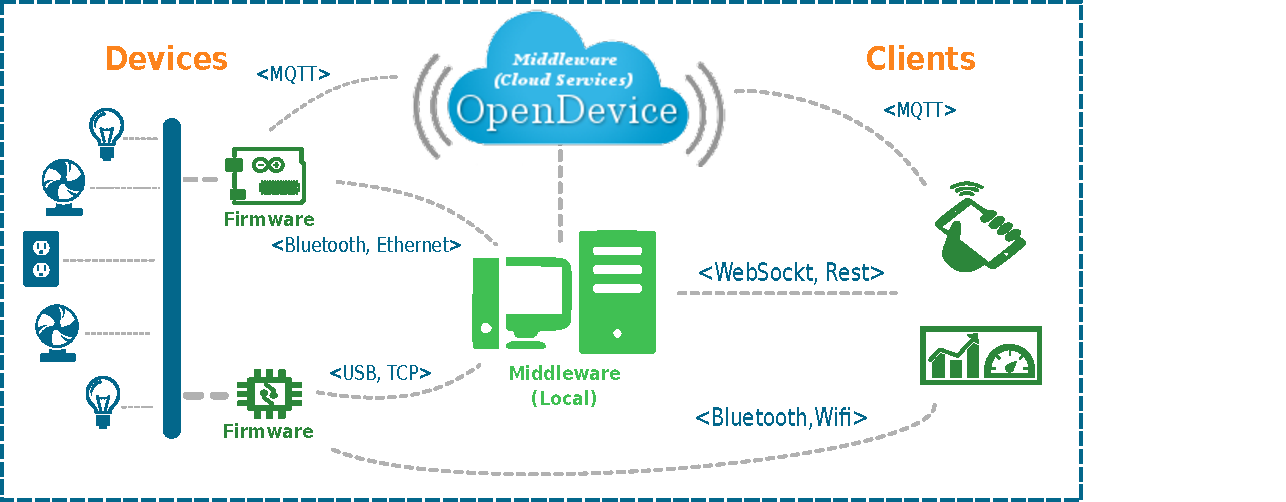
\includegraphics[width=1\linewidth]{Imagens/Cap_4/visao-geral}
\par\end{centering}
\caption{Visão Geral \label{fig:Visao-Geral}}
\end{figure}


\subsection{Componentes da Visão Geral\label{subsec:VisaoGeralComponentes}}
\begin{itemize}
\item \textbf{Middleware (Servidor)} - O middleware tem um papel fundamental
em projetos de IoT, como mencionamos na seção \ref{subsec:Fund_Middleware}.
No OpenDevice ele tem o papel de oferecer serviços para as aplicações
clientes, fazer o gerenciamento dos dispositivos, gerenciar múltiplas
conexões, fazer armazenamento e dispõe de módulos para visualização
dos dados através de dashboards dinâmicos e gráficos em tempo-real
ou históricos. Ele foi desenvolvido usando uma estrutura modular e
extensível, permitindo a inclusão de novos componentes e plug-ins
de maneira simplificada. Os desenvolvedores podem optar por utilizá-lo
como um servidor à parte, de modo embarcado ou estendendo-o. Esse
último é o modo aconselhado caso esteja desenvolvendo aplicações na
linguagem Java, pois sua arquitetura foi pensada como um framework,
de modo que os desenvolvedores de projetos de Internet das Coisas
incluam apenas as regras de negócio, sem se preocupar com os detalhes
de baixo nível. Projetos escritos em outras linguagens de programação
podem utilizar as APIs REST, MQTT, Socket e WebSocket para se comunicar
com os dispositivos através do middleware, que pode ser implantado
em um servidor local (PC / Raspberry Pi) ou na nuvem.O OpenDevice
suporta a criação de aplicações em JavaScript, que executam diretamente
na JVM (Java Virtual Machine), o que permite acesso aos módulos Java
e a criação de interfaces gráficas usando JavaFx.
\item \textbf{Firmware} - O firmware tem o papel de implementar o protocolo
do OpenDevice e fazer o gerenciamento dos dispositivos físicos (atuadores
e sensores) ligados a ele, criando uma abstração de alto nível, e
facilitando a integração com a camada de software. Nele, os dispositivos
(sensores e atuadores) são configurados e mapeados para um pino específico,
de modo que apenas as informações do dispositivo (ID, Nome, Tipo)
são expostas para as APIs externas, permitindo assim uma maior abstração
dos detalhes do hardware, ou até mesmo a substituição do hardware
por outro sem alterações na aplicação. Podemos pensar no firmware
também como um \emph{gateway,} responsável por manter a comunicação
com o middleware ou aplicação e controlar os dispositivos físicos.
É um componente de software projetado para rodar em dispositivos embarcados
com baixo poder de processamento e memória, algo em torno de 2KB de
RAM. O foco inicial do desenvolvimento foram os microcontroladores
encontrados em plataformas de prototipação como o Arduino e similares.
Com a expansão e popularidade da plataforma do Arduino inúmeros hardwares
estão dando suporte as suas APIs\cite{arduino-comp1,arduino-comp2},
ampliando a compatibilidade do firmware desenvolvido. Na seção \ref{par:Hardwares-Testados},
serão apresentados os hardwares testados. A arquitetura do firmware
é extensível, permitindo incluir novos dispositivos, novos comandos,
e suporte a novos tipos de conexões. Os detalhes do protocolo do OpenDevice
serão apresentados na seção \ref{subsec:Protocolo}. O Firmware é
um componente dispensável quando o projeto utilizar hardwares com
um maior poder de processamento e que tenham suporte a GPIO, como
no caso Raspberry ou BeagleBone. 
\item \textbf{Devices} - Representam os dispositivos físicos que podem ser
atuadores (representado pela classe \textbf{Device}) ou sensores (representados
pela classe \textbf{Sensor}). Estão organizados nos seguintes tipos:
(1) ANALOG, (2) DIGITAL, (3) CHARACTER, que estão ligados ao modo
de operação e tipo de dado suportado. Dentro do protocolo os dispositivos
são identificados através de um código, denominado DeviceID. Os dispositivos
do tipo ANALOG, podem receber uma faixa de valores numéricos, já os
dispositivos do tipo DIGITAL trabalham com dois estados: 0 (desligado)
e 1 (ligado), os dispositivos do tipo CHARACTER, estão aptos a receber
uma String. O OpenDevice trabalha com um modelo orientado a objetos,
permitindo que uma chamada dos métodos do \emph{Device} na aplicação
cliente, como por exemplo \emph{Device1.on()}, acenda uma lâmpada
real ou o realize fechamento de uma garra robótica. Eles podem ser
independentes ou estarem conectados a um microcontrolador, executando
o firmware, que faz o papel de Gateway. Os desenvolvedores podem estender
essa abstração e adicionar novos comportamentos para os dispositivos
e sensores.
\item \textbf{Clientes} - Representam as aplicações clientes, que podem
ser aplicações Desktop, web ou \emph{mobile} e podem ser desenvolvidas
em qualquer linguagem. As aplicações clientes, podem se comunicar
com o middleware, através das interfaces ofertadas (REST, MQTT, Socket,
WebSocket e etc.) ou diretamente com os dispositivos físicos. Foram
desenvolvidos módulos de bibliotecas clientes que permitem a integração
com o middleware em linguagens Java e JavaScript e experimentos de
integração usando a linguagem python. Mais detalhes sobre estas implementações
serão vistas na seção \ref{subsec:ConexoesCliente}. 
\end{itemize}

\subsection{Modelos de comunicação\label{subsec:ModelosComunicacao}}

A arquitetura planejada permite desenvolver projetos em vários Layouts
e modelos de comunicação, permitindo atender desde aplicações locais,
que se comunicam diretamente com os dispositivos, até aplicações distribuídas,
com comunicação através da internet.
\begin{itemize}
\item \textbf{Comunicação direta} - É um modelo que permite a comunicação
direta entre a aplicação final e os dispositivo físicos. Tem a característica
de ser mais simples, pois neste modelo, não se faz necessária a presença
do middleware (servidor). A aplicação neste cenário pode ser representada
por: (1) um dispositivo mobile, (2) uma aplicação desktop ou (3) uma
aplicação web. Representando o dispositivo físico, podemos ter um
hardware que disponibilize um mecanismo de comunicação embarcado,
por exemplo o ESP2866, que possui Wi-Fi, ou por exemplo um Arduino
com um módulo Bluetooth acoplado. Estes dois componentes podem se
comunicar usando diversas tecnologias, como: USB, Bluetooth, Ethernet,
Wi-Fi. Mais detalhes sobre os meios de comunicação e como eles são
implementados, serão vistos nas seções \ref{subsec:Arquitetura-do-Firmware}
e \ref{subsec:FirmwareGerenciamentoConn}.
\item \textbf{Comunicação local (Middleware)} - No modelo de comunicação
local, entre em cena um novo componente do OpenDevice, o middleware.
O middleware quando implantado dentro de um projeto pode ser visualizado
como o servidor, e pode ser configurado tanto em um computador convencional,
como em um mini-pc (ex.: Raspberry Pi). A vantagem da inclusão deste
elemento é que ele permite que diversas aplicações se comuniquem com
o mesmo dispositivo. Por exemplo, caso uma aplicação mobile esteja
conectada via Bluetooth com um dispositivo, outra aplicação será impedida
de se comunicar com esse dispositivo, usando middleware, essa limitação
é contornada, já que o middleware recebe os comandos das aplicações
cliente e faz o redirecionamento para o dispositivo desejado. Outra
vantagem é que o middleware pode gerenciar várias conexões com os
dispositivos, utilizando vários meios de comunicação, liberando essa
carga de gerenciamento das aplicações. Neste modelo de comunicação,
os dispositivos podem operar no modo servidor, aguardando a conexão
por parte do middleware, ou no modo cliente.
\item \textbf{Comunicação pela Internet} - Neste modelo as aplicações podem
se comunicar com os dispositivos através da internet. Para isso, os
dispositivos devem possuir um hardware que suporte uma conexão usando
o protocolo TCP/IP, necessitando apenas de um roteador convencional
para interligação com a internet ou um modem GSM/GPRS. Neste cenário
os dispositivos atuam no modo cliente e o middleware está implantado
em um servidor na nuvem.
\item \textbf{Comunicação pela Internet, usando um middleware local} - Neste
modelo um middleware local é aplicado novamente, permitindo que as
aplicações continuem funcionando caso a internet não esteja disponível
ou quando é necessário integrar dispositivos que não possuem suporte
o protocolo TCP/IP. Neste modelo, a mesma versão do middleware está
rodando em um servidor local e em um servidor na nuvem, diferenciando
apenas os módulos e infraestrutura utilizada, já que em um servidor
local a memória e recursos são limitados e num servidor de nuvem é
necessário uma performance e alta escalabilidade.
\end{itemize}

\subsection{Requisitos\label{subsec:Requisitos}}

A arquitetura foi projetada para ser adaptável às capacidades e necessidades
de casos de uso específicos. Esses podem ser categorizados como:
\begin{itemize}
\item \textbf{Requisitos de Comunicação} - O sistema deve ser apoiado em
eventos e/ou comunicação autônoma. Os dispositivos devem ser configurados
e controlados remotamente. O sistema deve suportar comunicação em
tempo-real. O sistema deverá fornecer comunicação segura e confiável.
O sistema deve prover recursos para extensão dos protocolos de comunicação.
\item \textbf{Gerenciamento de dispositivos} - A API deve prover uma interface
para o controle dos dispositivos. Isso inclui a configuração do dispositivo
bem como ativação, desativação e atualização remota.
\item \textbf{Serviços de Descoberta }- O sistema deve oferecer mecanismos
para descoberta e vinculação de novos dispositivos.
\item \textbf{Capacidades do dispositivo} - A API deve prover informações
sobre as capacidades dos dispositivos.
\item \textbf{Requisitos de comunicação cliente/servidor} - A API deve prover
suporte para operar os dispositivos tanto no modo cliente como no
modo servidor.
\item \textbf{Requisitos de monitoramento de status} - Status como nível
de bateria, temperatura, estado de operação dentro da infraestrutura
devem estar acessíveis.
\item \textbf{Serviço de Armazenamento} - A API deve oferecer recursos para
armazenamento das informações sobre os dispositivos, bem como mecanismo
para obter o histórico dos dados do dispositivo.
\item \textbf{Serviço de Visualização} - A API deve oferecer serviço para
análise dos dados, recursos para consultas históricas, funções para
agrupamento e agregação dos dados, bem como componentes visualização
através de gráficos.
\item \textbf{Orientado a Eventos} - O sistema deve oferecer um sistema
para tratamento de eventos, notificando as partes interessadas quando
alguma mudança de estado ocorrer nos dispositivos.
\item \textbf{Interoperável entre várias redes (PAN, LAN e WAN)} - Precisa
trabalhar através de uma variedade de redes e protocolos, tanto com
redes IP e não-IP, incluindo dispositivos de baixa potência (low-power)
em redes como Z-Wave, Zigbee e Bluetooth. 
\item \textbf{Extensível} - Deve fornecer recursos que permitam a inclusão
de novos componente e funcionalidades através de extensões ou plug-ins.
\item \textbf{Independência de Plataforma} - A API de serviços deve ser
multi-plataforma, executando nos principais sistema operacionais encontrados
no mercado.
\end{itemize}

\subsection{Extensibilidade\label{subsec:VisaoGeral-Extensibilidade}}

Toda a arquitetura do OpenDevice foi pensada visando uma fácil extensibilidade,
permitindo inclusão de novos protocolos, novos módulos de comunicação
e integração com outras ferramentas. Devido à grande diversidade de
áreas, requisitos e domínios variados que projetos de Internet das
Coisas podem ser empregadas, e por ser uma área relativamente nova,
é uma tarefa complexa desenvolver uma plataforma/Framework que atenda
a todos os requisitos. Esse trabalho oferece contribuições com uma
base sólida para criação de outros projetos especializados para outros
domínios como automação residencial, saúde, cidades inteligentes e
etc, porém sua estrutura generalista pode ser empregada para criar
vários projetos sem necessidade de modificações, no capítulo \ref{sec:Avaliacao-Experimental}
será realizada uma avaliação experimental, usando como base o domínio
da automação residencial para validar a arquitetura, com base na sua
aplicação generalista e nas suas capacidades de extensibilidade.

No contexto de extensibilidade, foram analisadas algumas estratégias
de implementação de suporte a plug-ins e módulos dinâmicos, uma das
soluções mais promissoras nesse campo é o OSGI (Open Services Gateway
Initiative)\cite{osgi}, porém foi descartado por considerarmos que
é uma ferramenta que adiciona uma complexidade extra no desenvolvimento
das extensões e necessita de um gerenciamento complexo que é feito
pelo contêiner de OSGI, consequentemente consumindo mais recursos.
A solução adotada é baseada em uma ferramenta disponível pela própria
linguagem Java, o SPI (Service Provider Interfaces), que tem como
objetivo, de oferecer recursos de extensão de forma simples e leve,
baseando-se apenas em interfaces que são definidas pelo próprio OpenDevice
e um arquivo de configuração simples. Uma pequena desvantagem encontrada
no mecanismo do SPI é que ele não permite o carregamento dinâmico
de plug-ins em tempo de execução, apenas no carregamento da aplicação.


\section{Arquitetura detalhada\label{subsec:Arquitetura-Detalhada}}

Nesta seção, veremos os detalhes da arquitetura empregada na construção
do projeto OpenDevice, analisando os módulos individualmente, os blocos
funcionais e suas responsabilidades.

Uma das considerações importantes no desenvolvimento desse projeto
é que o core da arquitetura e os módulos servidores principais~(MQTT,
Rest e WebSocket) pudessem ser executados em hardwares de baixo poder
de processamento, algo em torno de 512MB de RAM e 500Mhz de CPU. Com
base nessa restrição, foram desenvolvidos módulos de servidores que
executam em modo embarcado(\emph{embedded}), já que as soluções disponíveis
de servidores Java como: Tomcat , Jetty, JBoss ou GlassFish, iriam
consumir muitos recursos da máquina. O mesmo critério foi aplicado
na seleção do banco de dados, que é um componente opcional. Soluções
embarcadas foram adotadas em relação à soluções instaladas separadamente
(ex.: MySQL), facilitando o desenvolvimento e distribuição da aplicação.

A camada do middleware, das aplicações clientes e firmware são baseadas
no modelo de desenvolvimento orientado eventos (\emph{Event-Driven}),
realizada através do envio e recebimento de comandos, usando comunicações
em tempo-real. O modelo baseado em eventos facilita o desenvolvimento
de aplicações de IoT, principalmente quando é necessária a interação
com sensores, permitindo que os desenvolvedores registrem que tipo
de evento ou os dispositivos que desejam monitorar, e quando o evento
ocorrer, como por exemplo um sensor mudar seu valor, os interessados
no evento serão notificados. Esse modelo também permite uma fácil
extensão da ferramenta, pois tira a responsabilidade das extensões
de conhecer fluxo de conexão e aspectos internos do funcionamento,
podendo agregar funções mais elaboradas para lidar com os eventos,
como por exemplo, um algoritmo de inteligência artificial (IA) que
faça predição.

Na Figura \ref{fig:Arquitetura} pode-se observar a arquitetura e,
cada camada, assim como, cada elemento será explicado a seguir. 

\begin{figure}
\begin{centering}
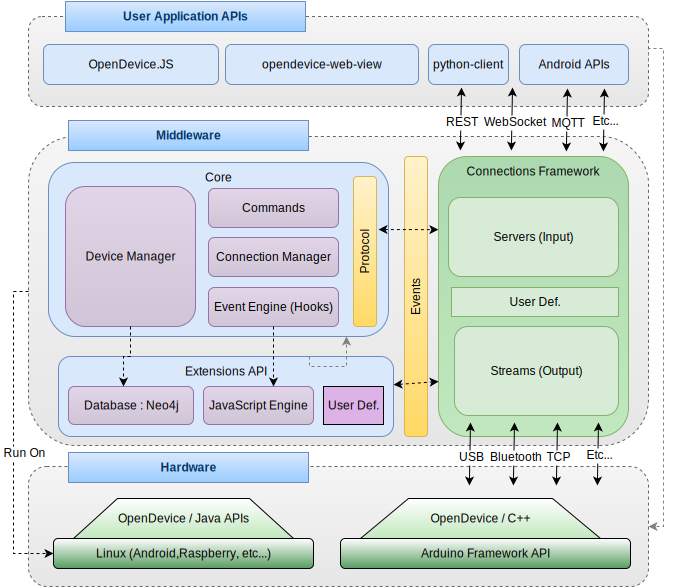
\includegraphics[width=1\linewidth]{Imagens/Cap_4/arquitetura}
\par\end{centering}
\caption{Arquitetura detalhada\label{fig:Arquitetura}}
\end{figure}


\subsection{Camadas da Arquitetura}
\begin{itemize}
\item \textbf{Camada de Aplicação (User Application APIs)} - Constituem
os módulos e bibliotecas disponibilizados para utilização pelas aplicações
clientes, permitindo a integração com o OpenDevice. A maioria dos
módulos são projetados para que as aplicações se comuniquem com os
dispositivos físicos (hardware) através do middleware, porém estão
disponíveis módulos que permitem a comunicação direta entre a aplicação
cliente e o hardware. Foram desenvolvidos módulos clientes para Web,
Desktop e Android, os detalhes da implementação e tecnologias suportadas
serão abordados na seção \ref{subsec:ConexoesCliente}.
\item \textbf{Middleware} - O middleware é uma camada altamente modular
e customizável, que oferece uma série de serviços para as aplicações,
como mencionamos na seção \ref{subsec:VisaoGeralComponentes} (Componentes
da Visão Geral). Ele é a peça central que permite a comunicação das
aplicações com os hardwares utilizando uma linguagem de alto-nível.
O middleware foi desenvolvido para uma fácil extensão, devido a essa
característica, ele se torna um framework para criação de projetos
de Internet das Coisas. Conta com um poderoso framework de conexões,
responsável pelas definições do protocolo, comunicação com os dispositivos
físicos e integração com as aplicações. Mais detalhes e sub-componentes
serão abordados a seguir.
\item \textbf{Hardware} - Os hardwares podem ser classificados em microcontroladores
e Mini PCs. Para os microcontroladores são disponibilizadas bibliotecas,
que chamamos nesse trabalho de firmware, que permitem uma fácil integração
com o middleware (servidor) e facilitam a criação de objetos inteligentes.
Elas dão suporte a utilização de várias tecnologias de comunicação,
como: Usb, Bluetooth, Ethernet e Wi-Fi. Essas bibliotecas são baseadas
no framework do Arduino, o que as tornam compatíveis com uma séries
de Hardwares e plataformas de prototipação, inclusive que não fazem
parte do projeto do Arduino\cite{arduino-comp1,arduino-comp2,arduino-comp3}.
Quando se trata de Mini PCs, que envolvem hardwares de maior poder
de processamento e memória, como por exemplo, Raspberry~Pi e BeagleBone,
é possível executar o middleware diretamente neles, desde que se tenha
disponível uma implementação da JVM para esses dispositivos. Nos Mini
PCs, o acesso aos pinos de GPIO ainda é um problema, pois cada hardware
possui suas especificações. O projeto Device I/O \cite{device-io:wiki},
mantido pela comunidade do OpenJDK, tem a proposta de criar uma implementação
para o acesso aos periféricos desses dispositivos, porém ainda está
em fase de desenvolvimento. Para hardwares não suportados pelo projeto,
existem três alternativas: (1) criar adaptadores/Wrapper para bibliotecas
já existentes, (2) implementar chamadas JNI ou (3) usar o drivers
baseados em \emph{Sysfs} que alguns Kernels disponibilizam para acessar
a GPIO como fossem simples arquivos\cite{key-sysfs}.
\end{itemize}

\subsection{Módulos}

Nesta seção, abordaremos os módulos que compõe a arquitetura. Na Figura
\ref{fig:Modulos} pode-se observar os módulos, assim como, cada elemento
será explicado a seguir. 

\begin{figure}
\begin{centering}
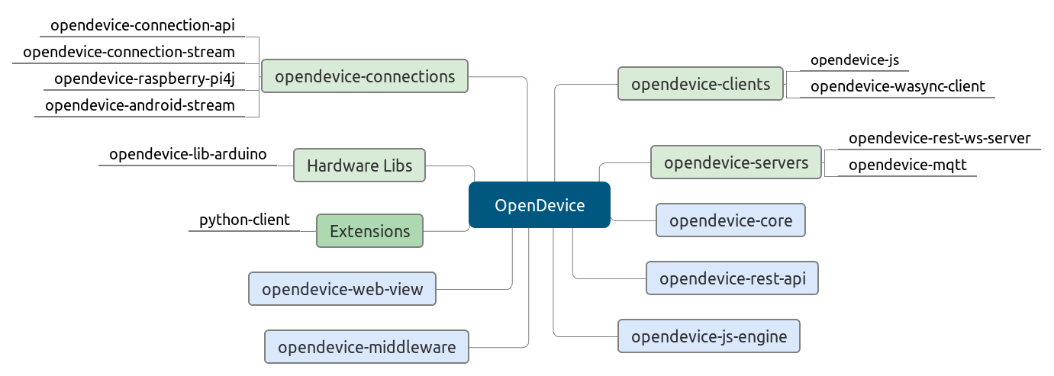
\includegraphics[width=1\textwidth]{/media/ricardo/Dados/Dropbox/Mestrado/Dissertacao/Imagens/Cap_4/OpenDevice_Modulos}
\par\end{centering}
\caption{Módulos\label{fig:Modulos}}
\end{figure}

\begin{enumerate}
\item Módulos Gerais

\begin{enumerate}
\item \noun{core}: Módulo base da arquitetura, com o sistema de gerenciamento
de dispositivos, sensores, conexões, eventos, armazenamento, API de
comandos e implementação do protocolo. Esse módulo pode ser usado
no desenvolvimento de aplicações Desktop, Web ou Mobile;
\item \noun{rest-api}: Definições das interfaces REST para controle dos
dispositivos e sensores;
\item \noun{js-engine: }Implementação do suporte a execução de JavaScript
no lado do servidor;
\item \noun{web-view}: Interface HTML/5 + AngularJS + OpenDeviceJS;
\item \noun{middleware: }Aplicação de gestão, controle e monitoramento,
que usa a maior parte dos módulos do OpenDevice, usando o banco de
dados Neo4J + Hibernate OGM (JPA).
\end{enumerate}
\item Módulos do framework de conexões

\begin{enumerate}
\item \noun{connection-api}: Especificação das interfaces de conexão cliente/servidor;
\item \noun{connection-stream}: Implementações de conexões USB, Bluetooth,
TCP (PC/RaspPI);
\item \noun{android-stream}: Implementação de conexões USB, Bluetooth para
Android\footnote{\begin{enumerate}
\item Demais conexões (Rest, WebSocket, MQTT) podem ser utilizada no Android
através dos outros módulos.
\end{enumerate}
};
\item \noun{raspberry-pi4j}: Comunicação com a GPIO do Raspberry usando
PI4J.
\end{enumerate}
\item Módulos Cliente

\begin{enumerate}
\item \noun{opendevice-js}: Biblioteca JavaScript com suporte a WebSocket
e REST;
\item \noun{opendevice-wasync-client}: Biblioteca WebSocket para Android
e PC;
\item \noun{python-client}: Biblioteca em Python com suporte a TCP.
\end{enumerate}
\item Módulos Servidores

\begin{enumerate}
\item \noun{rest-ws-server}: Servidor REST e WebSocket;
\item \noun{opendevice-mqtt}: Servidor MQTT;
\end{enumerate}
\item Bibliotecas para hardware

\begin{enumerate}
\item opendevice-lib-arduino: Bibliotecas em C++ baseadas na API do Arduino,
que implementa o protocolo do OpenDevice e são usadas para criação
do firmware. Provê suporte ao gerenciamento de dispositivos e conexões:
USB, Bluetooth, Wi-Fi, Ethernet. Veja a lista de placas testadas na
seção~\ref{par:Hardwares-Testados}.
\end{enumerate}
\end{enumerate}

\section{Gerenciamento de Dispositivos\label{sec:GerenciamentoDispositivos}}

Um dos principais requisitos de uma arquitetura de Internet das Coisas
é realizar a abstração dos dispositivos, permitindo lidar com a sua
grande heterogeneidade. No OpenDevice as abstrações base são implementadas
através das classes Device e Sensor. Algumas implementações de clientes
sofrem algumas variações nessa abstração, como por exemplo no cliente
JavaScript \noun{opendevice-js,} onde existe apenas a classe \emph{Device}
e a identificação, se é um sensor ou atuador, é feita através de um
atributo, já que nessa linguagem não temos suporte a orientação a
objetos. 

O OpenDevice permite a conexão com vários hardwares ao mesmo tempo,
cada hardware (ex.: Arduino) pode gerenciar vários sensores e atuadores,
cada sensor e atuador é interpretado como um ``\emph{Device}'' e
recebe um ID (DeviceID) único na plataforma, que pode ser codificado
manualmente ou dinamicamente. Quando o módulo cliente ou o middleware
estabelece uma conexão com o hardware (ex.: Arduino), ele solicita
as definições dos dispositivos que foram configurados. A biblioteca
(firmware) instalada no hardware, cuida de todo o processo de negociação.
A configuração de dispositivos no hardware pode ser feita de forma
estática, através de uma pre-configuração, ou dinâmica, através de
comandos. No hardware, os dispositivos são mapeados de forma a vincular
o pino do microcontrolador com um ID (DeviceID), de modo que as aplicações
externas conheçam o apenas ID, criando uma abstração do hardware final,
permitindo mudanças sem afetar a aplicação. Os hardwares, atuariam
como um Gateway, podendo ser identificados através de um nome ou ID,
e seriam responsáveis por controlar sensores e atuadores, e integra-los
às aplicações. 

A listagem \ref{alg:devices1} apresenta um exemplo (em Java) da configuração
dos dispositivos e conexão. Ao instanciar uma classe Device dentro
de uma classe que estende \emph{LocalDeviceManager, }eles passam a
ser gerenciados pelo OpenDevice, e qualquer alteração dos valores
dos dispositivos (ex.: \emph{led.on()} e \emph{led.off()}), resulta
em um envio de um comando para o hardware, que verifica o ID do dispositivo
e faz o mapeamento para o pino correspondente. No lado do hardware/firmware
(listagem \ref{alg:devices2}), a configuração dos dispositivos foi
realizada de forma estática, onde foram adicionados dois dispositivos:
(1) um atuador digital (led), conectado no pino 5 do Arduino e (2)
um sensor digital (switch), conectado no pino 3. A associação do ID
para cada dispositivo foi realizada de forma automática e sequencial,
porém é possível especificar um ID manualmente. 

Ao pressionar o sensor físico (ID=2), o firmware reconhece a alteração
no seu estado e envia uma notificação para a aplicação (ou middleware),
que chama o evento ``onChange'' do dispositivo especificado e notifica
outros componentes (incluindo extensões) que foram registrados para
esse evento. No evento disparado, no exemplo na listagem \ref{alg:devices1},
ele verifica o status atual do botão (linha 11), se estiver ligado/pressionado,
ele chama o método \emph{``on()''} do led. O OpenDevice detecta
essa alteração e envia o comando para o hardware (firmware) e este
faz o acionamento do pino correspondente ao dispositivo. Mais detalhes
sobre os fluxos de execução de comandos são apresentados na seção
\ref{subsec:FluxoMensagens}.

O exemplo apresentado demonstra a integração entre uma aplicação e
um hardware baseado em um microcontrolador, que tem um recursos extremamente
limitados. Em hardwares com maior poder de processamento, denominados
Mini-PCs (ex.: Raspberry), é possível executar a aplicação e fazer
o controle dos dispositivos diretamente, pois ele permite acesso aos
periféricos (pinos GPIO). A listagem \ref{alg:devices3}, apresenta
um exemplo resumido de como realizar o mapeamento dos dispositivos
para os pinos correspondentes do RaspberryPi.

\begin{algorithm}[H]
\inputencoding{latin9}\begin{lstlisting}[numbers=left]
// alguns trechos de c�digo foram omitidos
public class BlinkButtonDemo extends LocalDeviceManager{

    public BlinkButtonDemo() {

        final Device led = new Device(1, Device.DIGITAL);
        final Device btn = new Sensor(2, Device.DIGITAL);

        connect(out.bluetooth("00:13:03:14:19:07"));

        btn.onChange(device -> {
            if(btn.isON()){
                led.on();
            }else{
                led.off();
            }
        });
    }
}
\end{lstlisting}
\inputencoding{utf8}
\caption{Configuração dos dispositivos - Java\label{alg:devices1}}
\end{algorithm}

\begin{algorithm}[H]
\inputencoding{latin9}\begin{lstlisting}[language={C++}]
// alguns trechos de c�digo foram omitidos
void setup(){
    ODev.name("ModuleName");
    ODev.addDevice(5, Device::DIGITAL); // ID:1 - led 
    ODev.addSensor(3, Device::DIGITAL); // ID:2 - button
    ODev.begin(Serial1, 9600);
}

void loop(){
  ODev.loop();
}
\end{lstlisting}
\inputencoding{utf8}
\caption{Configuração dos dispositivos no Arduino - Firmware/C\label{alg:devices2}}
\end{algorithm}

\begin{algorithm}[H]
\inputencoding{latin9}\begin{lstlisting}[language={C++}]
// alguns trechos de c�digo foram omitidos
Device led = new Device(1, DeviceType.DIGITAL).gpio(1);
// ...
connect(new RaspberryGPIO());
\end{lstlisting}
\inputencoding{utf8}
\caption{Configuração dos dispositivos no Raspberry - Java \label{alg:devices3}}
\end{algorithm}


\section{Modelo Orientado a Eventos\label{sec:ModeloEventos}}

O design da arquitetura segue um modelo orientado a eventos, ou \emph{Event-Driven},
que permite desacoplar os componentes da arquitetura e aplicações.
Este desacoplamento pode ser de tempo, espaço ou sincronização\cite{key-eventd}. 

O mecanismo de eventos é importante na construção do framework, pois
ele é considerado mais eficiente e escalável do que o modelo baseado
em \emph{Polling}, que é um mecanismo síncrono de requisição e resposta,
que pode introduzir uma latência na comunicação e no tempo de resposta\cite{key-poll2}.
Esse mecanismo também permite a isolação das aplicações, de saber
qual a frequência com que os dispositivos geram os dados, passando
apenas a utilizar um mecanismo de ``observar'' os dispositivos,
e reagir aos eventos quando eles acontecem.

Os eventos gerados pelas aplicações clientes, são direcionados para
o middleware ou diretamente para os dispositivos, de forma automática
e transparente. Os principais eventos gerados pela arquitetura são:
mudança do estado do dispositivo, associação de novos dispositivos,
mudança no estado das conexões, porém exitem outros e novos podem
ser criados. È possível monitorar eventos gerados por dispositivos
individuais, registrado ouvintes (listeners) para as instâncias especificas,
ou para todos os dispositivos, registando ouvintes (listeners) no
gerenciador de dispositivos (\emph{DeviceManager}).

Um exemplo foi apresentado na seção \ref{sec:GerenciamentoDispositivos},
listagem \ref{alg:devices1}, onde é adicionado um ``ouvinte'' no
dispositivo e quando o valor dele mudar, o ``ouvinte'' é executado.
No exemplo citado, o ``ouvinte'' ao ser executado, faz a chamada
do método ``led.on()'', gerando um evento (comando) que é despachado
para os componentes interessados. Um dos interessados é o \emph{CommandDelivery},
que cuida do envio e monitoramento da entrega do comando, através
das conexões de saída. Outro interessado é o serviço de armazenamento
que, se habilitado, registra o histórico de alterações dos valores
dos dispositivos.

Algumas bibliotecas disponibilizadas para construção de aplicações
clientes se baseiam no sistema Publish/Subscribe, que permite um
baixo acoplamento e uma alta escalabilidade. Um dos exemplos é a
biblioteca JavaScript para desenvolvimento de aplicações WEB, \noun{opendevice-js},
que utiliza o procolo de comunicação WebSocket e consegue interagir
(envio e recebimento) com os dispositivos praticamente em tempo-real.


\section{API de Comandos\label{sec:APIComandos}}

As informações trocadas entre hardware, middleware e aplicações clientes
são baseadas em mensagens, que são chamadas de comandos e são representadas
pela classe base \emph{Command}. Esses comandos são convertidos no
protocolo do OpenDevice (mais detalhes serão vistos na seção \ref{subsec:Protocolo}),
através dos serializadores. O framework permite a comunicação com
os hardwares e controle dos dispositivos, utilizando apenas os comandos,
sem utilizar as abstrações obtidas com os dispositivos (classe \emph{Device}
e \emph{Sensor}). A listagem \ref{alg:command} mostra um exemplo
da equivalência da operação usando a classe \emph{Device} e usando
os comandos. A classe DeviceCommand, permite o envio de comandos do
tipo DIGITAL e ANALÓGICO. O recebimento de informações geradas pelo
hardware ou de outro componente (ex.:aplicação cliente), é realizada
através de comandos. Para realizar o monitoramento e recebimento desses
comandos é necessário adicionar os ouvintes (listeners) nas conexões,
um exemplo simplificado é apresentado na listagem \ref{alg:command-1}.
Ao enviar um comando para o hardware, ele irá responder com uma mensagem
de status, que é representada pela classe \emph{ResponseCommand},
permitindo identificar se os comandos foram recebidos corretamente
ou não. O envio das mensagens é gerenciado pelo \emph{CommandDelivery},
que permite direcionar a mensagem para a conexão certa e monitorar
a entrega. Caso ela não seja feita, devido a um delay ou falha de
comunicação, ele notifica a aplicação com um erro de \emph{timeout}
detalhes desse fluxo serão apresentados na seção \ref{subsec:FluxoMensagens}.
A figura \ref{fig:DiagCommands} mostra um diagrama de classe simplificado
da API de comandos. Essa API promove mais uma camada de abstração,
permitindo que, caso as implementações atuais dos dispositivos (Device
e Sensor) não sejam suficientes, elas possam ser substituídas.

\begin{algorithm}[H]
\inputencoding{latin9}\begin{lstlisting}[language={C++}]
// Usando a API de comandos
DeviceConnection conn = Connections.out.usb();
conn.send(DeviceCommand.ON(1)); // '1' is DeviceID

// Usando a abstra��o
Device led = new Device(1, Device.DIGITAL);
led.on();
\end{lstlisting}
\inputencoding{utf8}
\caption{Comparação da API de comandos e Devices \label{alg:command}}
\end{algorithm}

\begin{algorithm}[H]
\inputencoding{latin9}\begin{lstlisting}[language={C++}]
DeviceConnection conn = Connections.out.usb();
conn.addListener(new ConnectionListener() {
    public void onMessageReceived(Message message, DeviceConnection connection) {
        String type = message.getClass().getSimpleName();
        System.out.println("onMessageReceived("+type+"): "+ message);
    }
});
\end{lstlisting}
\inputencoding{utf8}
\caption{Monitorando recebimento de comandos \label{alg:command-1}}
\end{algorithm}

\begin{figure}
\begin{centering}
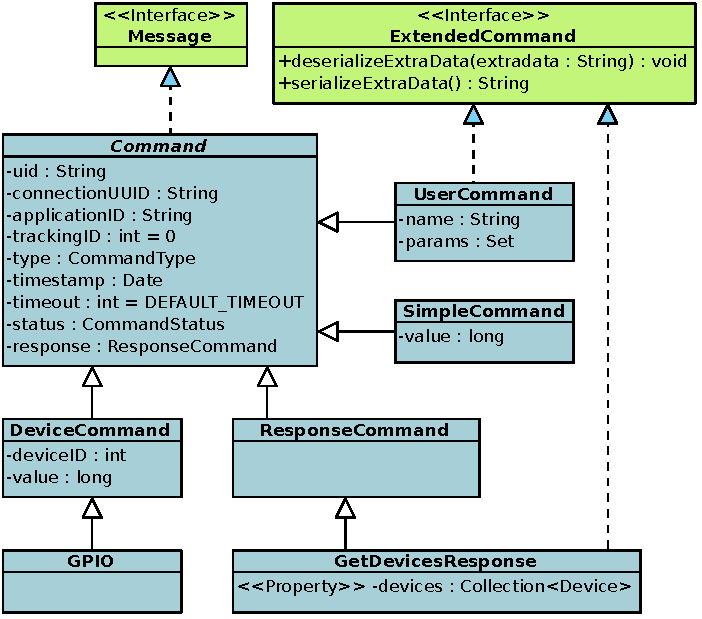
\includegraphics[width=0.7\linewidth]{Imagens/Cap_4/commands-api}
\par\end{centering}
\caption{Diagrama de classe simplificado dos Comandos\label{fig:DiagCommands}}
\end{figure}


\section{Mecanismo de extensão\label{sec:MecanismoExtensao}}

Como mencionado na seção \ref{subsec:VisaoGeral-Extensibilidade},
o mecanismo de extensão da arquitetura é baseado no SPI (Service Provider
Interface), um recurso simples e leve, disponível no Java 6 e posteriores.
Embora a arquitetura tenha sido projetada como um framework, para
ser usado como base para criação de projetos mais especializados,
existe uma implementação padrão, denominada \emph{middleware}, que
permite customizações através de extensões/plug-ins. Os mecanismos
de extensão padrão estão voltados para: (1) conexões, permitindo adicionar
novas conexões ou substituir por implementações mais eficientes, (2)
tratadores de eventos, que permitem plugar estratégias de tratamento
de eventos, e (3) sistema de armazenamento. As extensões são implementadas
através da interface \emph{OpenDeviceExtension}, que são inicializadas
durante o carregamento da aplicação. Para que as extensões sejam carregadas
corretamente é necessário que no módulo (.jar), seja incluído o arquivo
de configuração na pasta: \emph{resources/META-INF/services,} com
o nome:\emph{ br.com.criativasoft.opendevice.engine.js.ExtensionPoint},
seguindo as especificações do SPI. As conexões seguem um mecanismo
similar, porém possuem seus pontos de extensão individualizados para
cada tipo de conexão, como foi visto na figura \ref{fig:DiagConections}.


\subsection{Framework de Conexões\label{subsec:Framework-de-Conexoes}}

O framework de conexões foi projetado para ser usado de forma independente
do restante da arquitetura. A figura \ref{fig:DiagConections} mostra
a hierarquia base das conexões suportadas pela arquitetura. Essas
interfaces são os pontos de extensão, permitindo que implementações
possam ser utilizadas de acordo com a plataforma ou mesmo trocadas
por uma implementação mais eficiente. A figura \ref{fig:DiagConections2}
mostra um exemplo de implementação da conexão Bluetooth. A implementação
para aplicações Desktop é fornecida pelo módulo \noun{connection-stream},
já a implementação para aplicações Android são fornecidas pelo módulo
\noun{android-stream}, dessa maneira é possível que uma aplicação
possa ser portada sem modificações no seu código base para outras
plataformas. No OpenDevice a implementação correta é escolhida pela
fábrica de conexões, usando \emph{Connections.out.bluetooth(``...'').}
Esta fábrica está disponível no módulo core, e possui método para
criação das principais tecnologias de comunicação suportadas, tanto
clientes, como servidores. Os principais componentes desse framework
e suas descrições são listadas a seguir.

\begin{figure}
\begin{centering}
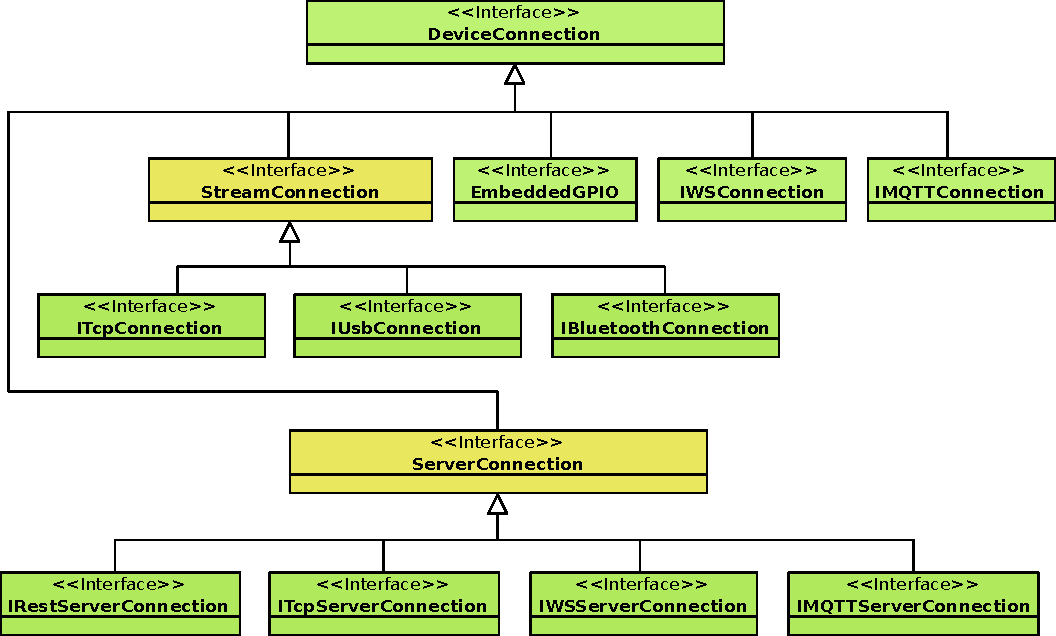
\includegraphics[width=1\linewidth]{Imagens/Cap_4/connections}
\par\end{centering}
\caption{Diagrama de classe das conexões\label{fig:DiagConections}}
\end{figure}

\begin{figure}
\begin{centering}
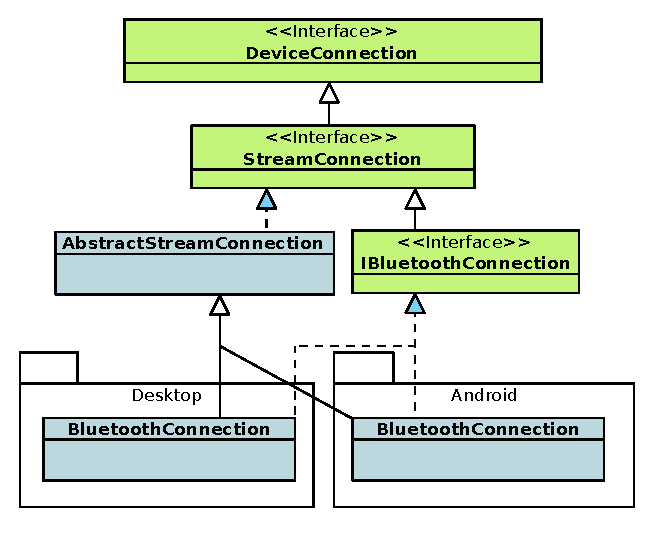
\includegraphics[width=0.7\linewidth]{Imagens/Cap_4/connections-bluetooth}
\par\end{centering}
\caption{Exemplo de implementação da conexão bluetooth\label{fig:DiagConections2}}
\end{figure}

\begin{itemize}
\item DeviceConnection - Interface base para todos as conexões do sistema,
define o modo de operação geral das conexões e em conjunto com o \emph{MessageSerializer}
define o modelo de protocolo a ser utilizado. Possui uma implementação
base, através da classe \emph{AbstractConnection}, que facilita a
criação de implementações finais. 
\item MessageSerializer - Como mencionado anteriormente, é o componente
responsável pela serialização e desserialização das mensagens enviadas
e recebidas pelas conexões. São as implementações que definem o tamanho
e formato das mensagens. A implementação padrão, localizada no módulo
core, é feita pela classe \emph{CommandStreamSerializer}. 
\item ConnectionListener - Interface que permite monitorar de forma plugável
os eventos ocorridos na conexão, como conexão, desconexão e recebimento
de mensagens, permitindo às aplicações reagirem à esses eventos. Vários
ouvintes de eventos (Listeners) podem ser adicionados àconexão.
\item Message - Interface que encapsula os dados enviados e recebidos, exemplos
de implementações são \emph{ByteMessage}, \emph{Request}, etc. A implementação
base usada no OpenDevice é realizada pela classe \emph{Command}, localizada
no módulo core.
\end{itemize}
No OpenDevice, esse framework é utilizado em duas camadas: (1) conexões
de entrada (Input), que são os servidores e têm por objetivo disponibilizar
os serviços para as aplicações clientes, como por exemplo o servidor
REST, e (2) conexões de saída (Output), denominados na maioria das
vezes como streams, que são as conexões com os módulos físicos (hardware)
e que implementam o protocolo de baixo nível, realizando a serialização
e desserialização dos comandos enviadas pelas aplicações. 

\section{Módulos Servidores \label{subsec:ConexoesServidores}}

Os módulos servidores, são responsáveis por fazer a interface com
as aplicações clientes. Eles permitem a inclusão de novos mecanismos
de conexão ou novos protocolos. Um exemplo de utilização de novo protocolo
é encontrado no servidor REST, que expande o protocolo do OpenDevice
(\ref{subsec:Protocolo}), permitindo criar interfaces mais simples
e de mais alto nível para as aplicações cliente se comunicarem com
os dispositivos.

O servidor WebSocket permite que aplicações (Web, Desktop, Mobile)
se comuniquem em tempo real e de forma bidirecional com os dispositivos,
usando middleware. O framework é projetado seguindo dois conceitos
de conexões: (1) conexões de entrada (Input), que são os servidores,
e (2) conexões de saída (Ouput), que são as conexões com os dispositivos
físicos. O papel do middleware é realizar a tradução dos protocolos
de entrada e converte-los para os protocolos de saída, específicos
para cada dispositivo, confirme a figura \ref{fig:middleware_connections}.
O módulo de visualização (com gráficos e dashboards), apresentado
na seção \ref{sec:Visualizacao}, utilizam as conexões em WebSocket
para permitir a comunicação em tempo-real com os dispositivos.

Os servidores permitem a abstração e desacoplamentos entre dispositivos
e aplicações, de modo que uma aplicação pode se comunicar com vários
dispositivos, ou permitir que varias aplicações se comuniquem com
o mesmo dispositivo, contornando alguns problemas das conexões que
suportam apenas um cliente, como no caso do Bluetooth e USB.

Os servidores foram projetados pensando na otimização de recursos
do hardware. Como o objetivo é permitir que eles possam executar em
hardwares, na categoria Mini-PCs, como o Raspberry e BeagleBone, as
implementações dos servidores utilizados no middleware, foram escolhidas
de modo que rodassem de forma embarcada e compartilhado o máximo de
recursos possíveis. Devido a arquitetura estar projetada para suportar
inicialmente os protocolos HTTP, Rest, WebSocket e MQTT, a implementações
dos mesmos seriam um desafio, devido a variedade de requisitos, estaria
fora do escopo da proposta deste trabalho. Foi então realizado um
estudo que mapeou as implementações desses protocolos individualmente,
e observou-se que as soluções mais maduras estavam baseadas em frameworks
de rede. Os principais frameworks encontrados foram: Jetty (Eclipse)\footnote{http://www.eclipse.org/jetty/},
Grizzly (GlassFish)\footnote{https://grizzly.java.net} e Netty\footnote{http://netty.io}.
O Jetty é um contêiner de aplicações Java e servidor web, que tem
uma estrutura modular e suporta protocolos como Http e WebSocket.
Apesar ser possível executar de forma embarcada, sua estrutura foi
planejada para executar aplicações Java web (.war), não como um framework
genérico e nem com plataformas embarcadas em mente. O Grizzly por
sua vez é projetado como um framework, e utilizado como base na construção
do servidor de aplicação GlassFish, suportando também HTTP, WebSocket
e sendo de fácil extensão. Por fim, o Netty, é também um framework
que tem uma estrutura simples, é utilizado para construção de projetos
como Apache Spark, Elasticsearch, Neo4j (banco de dados), Minecraft
e outros\footnote{http://netty.io/wiki/adopters.html}. O Netty é
framework utilizado como base das implementações dos servidores escolhidos
para o projeto arquitetura. 

A escalabilidade da arquitetura pode ser alcançada, substituindo os
implementações dos servidores embarcados, por implementações mais
robustas, que permitam escalonamento horizontal e balanceamento de
carga. Isto pode ser alcançado, de forma transparente para a aplicação,
utilizando os mecanismos de extensão (\ref{subsec:VisaoGeral-Extensibilidade},
\ref{sec:MecanismoExtensao}).

\begin{figure}
\begin{centering}
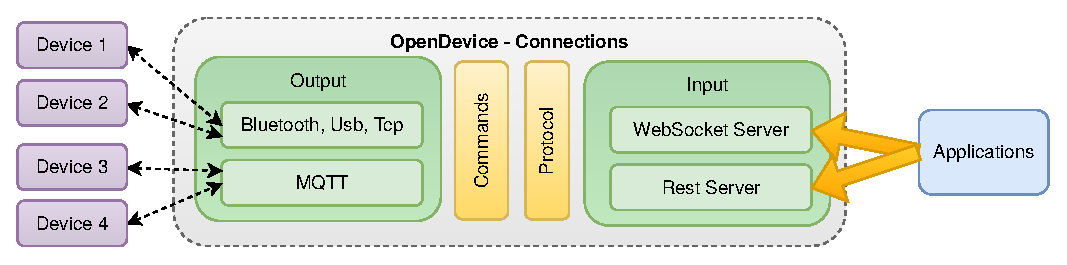
\includegraphics[width=0.8\linewidth]{Imagens/Cap_4/middleware_connections}
\par\end{centering}
\caption{Abstração dos protocolos de comunicação\label{fig:middleware_connections}}
\end{figure}


\subsection{Servidor MQTT}

A implementação de servidor MQTT escolhida, foi o ``Moquette MQTT'',
projeto mantido pela fundação Eclipse, e que utiliza como base o framework
de rede Netty.

Os servidores são em sua maioria destinados à comunicação com as aplicações
clientes (conexões de entrada). O MQTT é uma exceção, pois permite
que os dispositivos físicos também sejam conectados ao middleware.
Para permitir um gerenciamento e integração com o middleware, e permitir
a comunicação bidirecional entre aplicações e dispositivos físicos,
algumas convenções foram adotadas na nomenclaturas dos tópicos. 

Tanto as aplicações como os dispositivos físicos são ``publish''
e ``subscriber''. O middleware é o encarregado de monitorar as mensagens
e fazer o direcionamento adequado, atuando como espécie de ``subscriber''
geral. Caso uma aplicação envie uma requisição para um dispositivo,
é papel do middleware fazer o direcionamento para o tópico correto,
e monitorar a resposta e envia-la de volta (publish) para a aplicação
que fez a requisição. A camada das aplicações não conhecem a estrutura
de tópicos do borker MQTT e seu mapeamento para os dispositivos, elas
apenas possuem as abstrações dos dispositivos, orientadas a objetos,
e enviam os comandos para o middleware (ex.: device.on()). Isso mermite
que aplicações clientes MQTT consigam se comunicar com dispositivos
Bluetooth e MQTT de forma transparente.

A tabela \ref{tab:mqtt_nomenclatura}, apresenta as nomenclaturas
estabelecias para o nome dos tópicos. Quando uma aplicação realiza
uma operação na abstração do dispositivo (ex.: device.on()), um comando
é enviado para tópico ``ProjectID/middeware/in'', que é o canal
que o middleware usa para o recebimento dos comandos das aplicações.
Na implementação atual, por ser embarcada, o recebimento é feito diretamente
sem necessidade do middleware se inscrever nos tópicos. O middleware
identifica o dispositivo e determina qual conexão que o dispositivo
em questão está vinculado, que pode ser uma conexão Bluetooth ou MQTT,
nesse ultimo caso, o firmware envia (publish) o comando para seu respectivo
tópico: ``ProjectID/in/ModuleName''.

O componente denominado ``Firmware'' é um hardware (ex.: arduino)
que pode estar gerenciando um ou mais dispositivos (sensores e atuadores),
onde internamente cada um recebe uma identificação (DeviceID). Cada
conexão com um hardware recebe uma identificação chamada ``ModuleName''.

\begin{table}[h]
\begin{centering}
\begin{tabular}{|c|c|c|c|}
\hline 
Componente & Operação & Tópico & Descrição\tabularnewline
\hline 
\hline 
Firmware & Publish & ProjectID/out & Envio de Dados\tabularnewline
\hline 
Firmware & Subscribe & ProjectID/in/ModuleName & Recebimento de comandos\tabularnewline
\hline 
Middleware & Subscribe{*} & ProjectID/out & {*} Monitoramento (Listener)\tabularnewline
\hline 
Middleware & Subscribe{*} & ProjectID/middeware/in & {*} Monitoramento (Listener)\tabularnewline
\hline 
App & Publish & ProjectID/middeware/in & Envio de Comandos\tabularnewline
\hline 
App & Subscribe & ProjectID/middeware/out & Notificações Gerais\tabularnewline
\hline 
App & Subscribe & ProjectID/middeware/out/CID & Tópico de Resposta\tabularnewline
\hline 
\end{tabular}
\par\end{centering}
\caption{Nomenclatura de tópicos MQTT\label{tab:mqtt_nomenclatura}}
\end{table}


\subsection{Servidores WebSocket, Rest e Http}

O WebSocket é o protocolo originalmente utilizado para permitir a
comunicação em tempo-real com as aplicações Web, porém é possível
a sua utilização em aplicações Desktop. A implementação desse protocolo
é fornecida pelo projeto Nettosphere\footnote{https://github.com/Atmosphere/nettosphere},
também baseado no framework Netty. O grande diferencial é que ele
oferece a implementação dos três protocolos utilizando a mesma porta
(ex.: 80), e consequentemente poupando muitos recursos do hardware.
Isso é possível devido a estrutura de processamento do framework Netty,
que permite identificar e processar cada protocolo separadamente.
Teoricamente o mesmo poderia ser feito para o protocolo MQTT, mas
seria um desafio atingir o nível de maturidade da implementação embarcada
que adotamos.

O servidor HTTP, permite a configuração de pastas de recursos como
HTML, CSS e imagens, permitindo a criação de interfaces gráficas.

O servidor REST, permite a criação de serviços que atendem ao protocolo
REST. A integração com o Jesey\footnote{https://jersey.java.net},
permite a implementação da especificação Java \emph{(JAX-RS - The
Java API for RESTful Web Services}), facilitando e padronizando a
criação de novos serviços, estendendo as capacidades do \emph{middleware}.
Os serviços Rest criados, contam com suporte a injeção de dependências,
seguindo a especificação JSR-330, que se utilizam das anotações \emph{@Inject
e @Named}, para injeção dos componentes.

\section{Suporte a JavaScript\label{subsec:SuporteJavaScript}}

O suporte a JavaScript permite a criação de aplicações simples e tratadores
de eventos, que rodam nativamente, e é integrado ao OpenDevice através
do mecanismo de extensões. Também é possível criar aplicações Web,
utilizando JavaScript, com auxílio da biblioteca \noun{opendevice-js,
}que permite a abstração dos dispositivos e implementa os protocolos
REST e WebSocket.

No primeiro caso, é possível criar aplicações que executa nativamente,
ou seja, sem depender de um navegador, pois rodam diretamente na JVM,
Este suporte é fornecido através do módulo \noun{js-engine}, que usa
os recursos da própria JVM implementados no projeto Nashorn \footnote{http://openjdk.java.net/projects/nashorn/}.
Este recurso auxilia na sua utilização por desenvolvedores que não
têm experiência com linguagem Java ou mesmo desenvolvedores experientes
que precisam realizar uma prototipação mais rápida ou pela simplicidade
da implementação de tratamento de eventos com uma linguagem de script.
Devido a necessidade de recursos avançados da JVM, esse módulo (\noun{js-engine})
depende da versão Java 8, que inclui várias melhorias de performance
e integração com JavaScript. Os modos de desenvolvimento serão detalhados
a seguir.

\subsection{Criação de aplicações nativas em JavaScript}

As aplicações criadas em JavaScript, executam na JVM e têm interoperabilidade
com as classes definidas em Java. Desse modo é possível realizar chamadas
nas classes e métodos do OpenDevice. A listagem \ref{alg:ExemploJS1},
demonstra um exemplo de criação de uma aplicação simples, que ao detectar
uma mudança no botão~(BUTTON), controla o estado da lâmpada~(led).
O módulo \noun{js-engine} pode ser compilado para um executável (odevjs.exe
ou odevjs.jar), destinado a execução de aplicações em JavaScript usando
o comando: \inputencoding{latin9}\lstinline!> odevjs.exe myscript.js!\inputencoding{utf8}.

Outro exemplo de aplicação, usando interface gráfica (GUI) em JavaFX,
pode ser encontrado no Apêndice \ref{chap:ApendiceA}. Para habilitar
o JavaFX é necessário informar o parâmetro ``-fx'', exemplo: \inputencoding{latin9}\lstinline!> odevjs.exe -fx myscript.js!\inputencoding{utf8}.
Os códigos JS podem ser executados diretamente de aplicações Java,
através da classe \emph{OpenDeviceJSEngine}, exemplo: \inputencoding{latin9}\lstinline!OpenDeviceJSEngine.run("myscript.js")!\inputencoding{utf8}.

\begin{algorithm}[H]
\inputencoding{latin9}\begin{lstlisting}
var led = new Device(1, DIGITAL);
var button = new Sensor(2, DIGITAL);

button.onChange(function(){
    if(button.isON()){
        led.on();
    }else{
        led.off();
    }
});

connect(usb());
\end{lstlisting}
\inputencoding{utf8}
\caption{Exemplo de Aplicação em JavaScript\label{alg:ExemploJS1}}

\end{algorithm}


\subsection{Tratadores de Eventos (EventHook)}

Os tratadores de evento (EventHook), são pequenos trechos de código
JavaScript que estão vinculados os dispositivos (Devices e Sensors)
e são executados quando acontece alguma mudança do seu valor. Esse
mecanismo é uma extensão para o EventManager, e implementada pela
classe \emph{JavaScriptEventHandler}. A implementação padrão faz o
carregamento dos scripts através de arquivos, mas pode-se implementar
outras formas de armazenamento/carregamento. Na implementação atual
os eventos são mapeados para os dispositivos através de metadados
incluídos no próprio script. Na listagem \ref{alg:ExemploJS2}, é
implementado a mesma lógica da listagem \ref{alg:ExemploJS1}, entretanto,
eles não são interpretados através do executável (odevjs.exe), eles
são gerenciados pelo middleware e são executados quando os dispositivos
mapeados através da anotação \noun{@devices,} sofrem alguma modificação.
A variável ``device'', é injetada pelo framework e representa o
dispositivo que sofreu a alteração.

\begin{algorithm}[H]
\inputencoding{latin9}\begin{lstlisting}[language=VBScript]
/**
 * @name ButtonHookDemo
 * @devices 2
 * @description TestCase
 * @type JavaScript
 */
var led = findDevice(1);
if(device.isON()){
    led.on();
}else{
    led.off();
}
\end{lstlisting}
\inputencoding{utf8}
\caption{Exemplo do ``EventHook'' em JavaScript\label{alg:ExemploJS2}}
\end{algorithm}


\subsection{Criação de aplicações WEB em JavaScript}

A biblioteca \noun{opendevice-js} foi desenvolvida para auxiliar no
desenvolvimento de aplicações Web escritas em qualquer outra linguagem,
e sua integração com os dispositivos físicos. Ela permite a comunicação
em tempo real com os dispositivos graças ao suporte a WebSocket. Trabalha
no modelo orientado a eventos, ou seja, quando ocorre alguma mudança
no estado no dispositivo, o evento ``\emph{onChange}'' é chamado,
conforme no exemplo na listagem \ref{alg:ExemploJS3}. Ela é utilizada
na construção do \emph{Front-End Web} do middleware (\ref{sec:Visualizacao}),
que permite fazer o controle dos dispositivos, realizar a análise
e visualização de dados em tempo-real ou de dados históricos. 

\begin{algorithm}[H]
\inputencoding{latin9}\begin{lstlisting}[language=VBScript]
<script>
    $(function(){ // JQuery ready()
        ODev.connect();
    });

    ODev.onChange(function(device){
        if(device.sensor){
            ODev.findDevice(1).setValue(device.value);
        }
    });
</script>
\end{lstlisting}
\inputencoding{utf8}
\caption{Exemplo de utilização da biblioteca \noun{opendevice-js}\label{alg:ExemploJS3}}
\end{algorithm}


\section{Visualização e controle dos dispositivos\label{sec:Visualizacao}}

O middleware conta uma uma interface Web (figura \ref{fig:dashboard1}
e \ref{fig:dashboard2}), desenvolvida em HTML5 e AngularJS, e é implementado
pelo módulo \noun{opendevice-web-view, }que permite o monitoramento,
controle dos dispositivos e visualização do dados através de gráficos
e indicadores. A visualização pode ser em tempo-real ou através de
consultas a dados históricos. É possível aplicar funções como: (1)
média, (2) mínimo, 3 (máximo), 4 (soma), 5 (contagem) e 6 (desvio
padrão), nos dados de um determinado intervalo que é configurado via
a interface gráfica. Os gráficos implementados são: (1) gráfico de
linha, (2) gráfico de pizza, (3) gauge e (4) indicador numérico. Os
\emph{dashboards} são altamente flexíveis, permitindo configurar o
tamanho, adicionar e remover gráficos. Alguns gráficos permitem a
inclusão de vários dispositivos, permitindo uma análise comparativa,
como no exemplo da figura \ref{fig:dashboard2} (Luz Semana 1), foram
incluídos três dispositivos em um gráfico de linha. O mesmo permite
funções de zoom em determinado período de forma interativa. Os dashboards
permitem também a inclusão de dispositivos e sensores digitais, permitindo
o controle, ativação, desativação e visualização do status atual.

\begin{figure}[H]
\begin{centering}
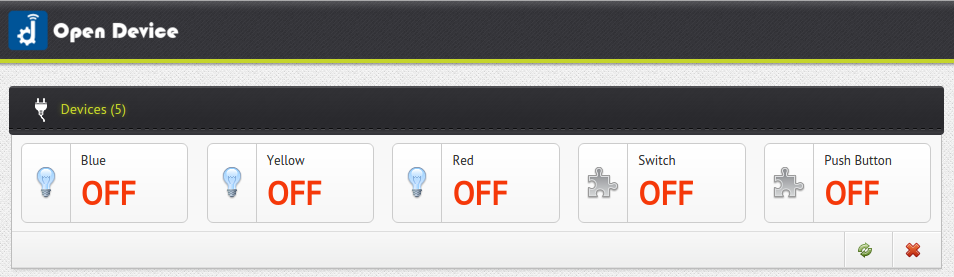
\includegraphics[width=1\linewidth]{Imagens/Cap_4/dashboard-devices}
\par\end{centering}
\caption{Interface de controle de dispositivos\label{fig:dashboard1}}
\end{figure}

\begin{figure}[H]
\begin{centering}
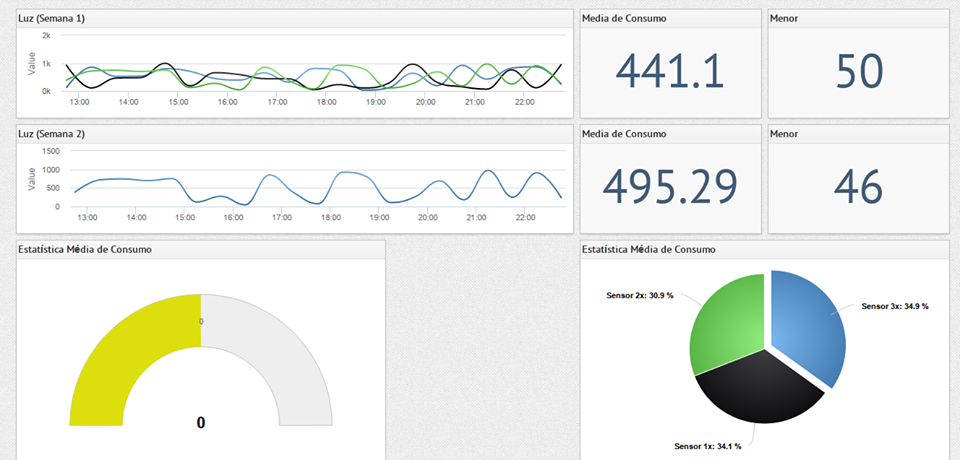
\includegraphics[width=1\linewidth]{Imagens/Cap_4/dashboard-charts}
\par\end{centering}
\caption{Interface de Dashboards Gráficos\label{fig:dashboard2}}
\end{figure}


\section{Serviço de descoberta\label{sec:ServicoDescoberta}}

Conectar e configurar um dispositivo (microcontrolador, sensor ou
atuador), é uma tarefa relativamente simples. Fazer o mesmo para centenas
ou milhares de dispositivos, não é uma tarefa fácil. Este é o cenário
que os pesquisadores e desenvolvedores irão encontrar no ambiente
de Internet das Coisas. Um mecanismo dinâmico, adaptável e utilizando
um processo mais automatizado possível, é necessário para realizar
a descoberta de dispositivos e registro de suas informações básicas.
Além disso existe a necessidade de trabalhar de forma unificada com
diferentes protocolos e dispositivos de rede.

O framework conta com serviços de descoberta de dispositivos, suportando
as tecnologias Usb, Bluetooth, Ethernet e Wi-Fi. O middleware também
disponibiliza um serviço de descoberta, permitindo que as aplicações
clientes o localizem em uma rede local. São dois os possíveis cenários
onde as aplicações e dispositivos IoT estarão executando: Local e
Internet. No cenário onde os dispositivos estão conectados à Internet,
eles devem ser configurados para atuarem como clientes, conectando-se
no servidor em nuvem do OpenDevice em um endereço fixo. Já em um cenário
local, focando-se em dispositivos Ethernet, no cenário de automação
residencial, por exemplo, os dispositivos poderiam atuar em modo cliente
ou como servidor, em ambos os cenários seria necessário configurar
manualmente um IP fixo para cada dispositivo, uma tarefa relativamente
trabalhosa dependendo da quantidade de dispositivos.

Uma solução promissora é o padrão DNS-SD (DNS Service Discovery, RFC
6763) \cite{key-dnssd}, que permite a descoberta de serviços na rede
e associação de um ``DNS local'' para o dispositivo, como por exemplo:
\emph{lampada1.local}. Devido às limitações de alguns hardwares alvos
do estudo (microcontroladores), uma solução mais simples foi adotada.
Trata-se do envio de mensagens UDP em broadcast na rede. Os dispositivos
(hardware) monitoram a rede e ao detectar uma solicitação de descoberta
(um comando do tipo \emph{DISCOVERY\_REQUEST}), enviam uma mensagem
de volta contendo o seu nome, tipo, IP atual, e porta. Desse modo,
todos os dispositivos podem ser configurados com IP dinâmico usando
DHCP, incluindo o próprio servidor (middleware). As aplicações clientes
podem localizar os dispositivos ou middleware utilizando o mesmo mecanismo. 

Foi desenvolvida uma estratégia bastante simples, influenciada pelo
DNS-SD e combinado com a técnica desenvolvida, para conexão com os
dispositivos TCP/IP, usando um endereço com sufixo pré-definido (ex.:
\emph{lampada1}.local.opendevice). A listagem \ref{alg:descoberta}
apresenta um modelo tradicional de descoberta e o modelo usando os
endereços de domínio local. No primeiro exemplo (modelo tradicional)
é obtido o serviço de descoberta e iniciado a busca durante 5 segundos
por dispositivos na rede, em seguida é feita a conexão. No segundo
exemplo, ele permite a simplificação do processo. O endereço informado
``lampada1.local.opendevice'', na verdade não se trata de um domínio,
serve apenas para marcar e iniciar o sistema de descoberta automático,
permitindo uma fácil conexão com determinado dispositivo (hardware).
A imagem \ref{fig:DiagDiscoveryConnect} apresenta um diagrama de
fluxo de como esse processo funciona.

As conexões USB e Bluetooth, possuem mecanismos de descobertas menos
sofisticados, oferecidos pelas próprias implementações no S.O, que
são usados pelo serviço de descoberta. No caso do USB, a classe que
implementa essa conexão (\emph{UsbConnection}), possui o método ``listAvailable'',
que lista todos os dispositivos USB-Serial conectados na maquina.
É possível realizar facilmente uma conexão com o primeiro dispositivo
encontrado usando: \inputencoding{latin9}\lstinline!connect(out.usb())!\inputencoding{utf8}.
A implementação para Bluetooth é similar, onde o método ``listAvailable''
da classe (\emph{BluetoothConnection}), realiza a listagem dos dispositivos
seriais SSP - (Serial Port Profile) disponíveis, também é possível
conectar-se facilmente com o primeiro dispositivo encontrado, usando:
\inputencoding{latin9}\lstinline!connect(out.bluetooth())!\inputencoding{utf8}
(observe que, antes é necessário realizar manualmente o pareamento
dos dispositivos). 

\begin{algorithm}[H]
\inputencoding{latin9}\begin{lstlisting}[language={C++}]
// Modelo tradicional
Set<NetworkDeviceInfo> devices = getDiscoveryService().scan(5000, null);
if(devices.size() > 0){
    NetworkDeviceInfo info = devices.iterator().next();
    if(info.getName().equals("lampada1")) {
        connect(out.tcp(info.getIp() + ":" + info.getPort()));
    }
}

// Modelo usando dom�nio local
connect(out.tcp("lampada1.local.opendevice"));
\end{lstlisting}
\inputencoding{utf8}
\caption{Exemplos de descoberta de dispositivos \label{alg:descoberta}}
\end{algorithm}

\begin{figure}
\begin{centering}
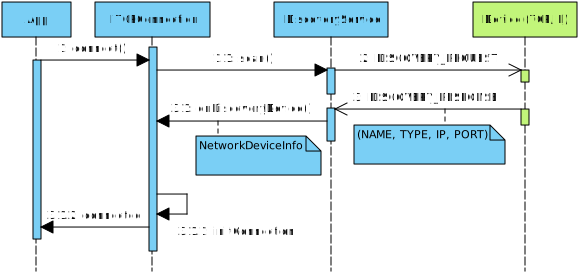
\includegraphics[width=0.8\linewidth]{Imagens/Cap_4/seq_discovery_connect}
\par\end{centering}
\caption{Fluxo de conexão e descoberta\label{fig:DiagDiscoveryConnect}}
\end{figure}


\section{APIs para Aplicações Cliente\label{subsec:ConexoesCliente}}

O conjunto de bibliotecas ou APIs para aplicações clientes, permitem
a rápida construção de aplicações, sem que os pesquisadores ou desenvolvedores
tenham que se preocupar com os detalhes de baixo nível do protocolo,
adotando um modelo orientado a eventos (\emph{Event-Driven}) e usando
orientação a objetos na construção das aplicações, que podem ser aplicações
Web, Desktop, Mobile ou uma interface simulação. O maior desafio encontrado
na construção dessas aplicações é lidar com a heterogeneidade dos
dispositivos (atuadores e sensores), fazer o gerenciamento das conexões
e a integração com a aplicação. A arquitetura disponibiliza um middleware
e um framework para construção aplicações ou middleware customizadas.

As bibliotecas disponibilizadas permitem uma comunicação bidirecional
e são focadas na comunicação em tempo real, dessa maneira é possível
construir gráficos para visualização das informações em tempo-real,
aplicações de simulação, etc. As tecnologias empregadas que permitem
essa comunicação, estão disponíveis para as plataformas Web, Desktop
e Mobile, conforme a tabela \ref{tab:apis-clientes}.

\begin{table}[h]
\begin{centering}
\begin{tabular}{|c|c|c|c|c|}
\hline 
Tipo & Web & Desktop & Mobile (Android) & Alvo de Comunicação\tabularnewline
\hline 
\hline 
USB &  & X &  & Firmware\tabularnewline
\hline 
Bluetooth &  & X & X & Firmware\tabularnewline
\hline 
Socket (TCP) &  & X &  & Middleware/Firmware\tabularnewline
\hline 
WebSocket & X & X & X & Middleware\tabularnewline
\hline 
MQTT &  & X & X & Middleware\tabularnewline
\hline 
\end{tabular}
\par\end{centering}
\caption{APIs Clientes\label{tab:apis-clientes}}
\end{table}


\subsection{Implementação}

A maior parte das bibliotecas são implementados em linguagem Java
com base no framework de conexões (\ref{subsec:Framework-de-Conexoes})
e utilizam o módulo principal (core), que provê as APIs de comandos
e abstração de dispositivos. Porém são disponibilizadas bibliotecas
em JavaScript, apresentada na seção \ref{subsec:SuporteJavaScript},
e Python (experimental). As tecnologias de comunicação (ex.: USB),
são implementadas com auxílio de bibliotecas externas, e suas considerações
são listadas a seguir.

\subsubsection{USB}

A comunicação USB, por utilizar recursos do sistema operacional e
ser dependente da arquitetura, não possui suporte nativo na JVM, apesar
de ser umas das especificações iniciais da plataforma, registrada
sobre a especificação Java USB API (JSR-80)\cite{key-JSR-80}.

Como alternativa, algumas bibliotecas de terceiros foram avaliadas.
Uma das pioneiras e mais utilizadas é a biblioteca RXTX\footnote{https://github.com/rxtx/rxtx}.
Esta biblioteca foi utilizada nas versões iniciais da plataforma,
porém, pelo fato de não ter um desenvolvimento ativo, e nos testes
realizados ter se mostrado instável, apresentando alguns erros (ex.:
problemas de deadlocks e mal funcionamento em plataformas ARM), ela
foi substituída.. A implementação de referência oficial, javax-usb
\footnote{http://javax-usb.sourceforge.net/}, a julgar pelo site
e documentação, estão abandonados há muito tempo.

A implementação utilizada, foi baseada na biblioteca JSSC (Java Simple
Serial Connector)\footnote{https://github.com/scream3r/java-simple-serial-connector},
que oferece suporte para várias plataformas\footnote{Segundo o site: Windows(x86, x86-64), Linux(x86, x86-64, ARM soft
\& hard float), Solaris(x86, x86-64), Mac OS X(x86, x86-64, PPC, PPC64)}, se mostrando uma alternativa promissora. Ela é a biblioteca utilizada
na IDE do Arduino, substituindo a RXTX em versões anteriores.


\subsubsection{Bluetooth}

A comunicação Bluetooth é apoiada na especificação Java JSR-82\cite{key-JSR-82},
possui implementações bem estabelecidas e estáveis para o desenvolvimento
para dispositivos móveis, usando JavaME. As implementações para ambiente
desktop, sofrem com os mesmos problemas de plataforma do USB. Uma
das poucas alternativas, é a biblioteca BlueCove\footnote{http://bluecove.org/},
que tem implementações para os principais sistemas operacionais (Windows,
Linux, MacOS). Para o suporte à plataformas ARM (no RaspberryPi),
foi necessário a recompilação da mesma e ajustes, pois não foram encontradas
versões disponibilizadas no site oficial nem de terceiros. 

As implementações para aplicações mobile, estão disponíveis para o
Android, e utiliza as APIs disponibilizadas pela própria plataforma.
A arquitetura do OpenDevice, é projetada de maneira que a implementação
utilizada é transparente para o desenvolvedor, sem precisar de modificações
no código.

\subsubsection{Socket (TCP)}

Foi implementada usando as APIs nativas do Java, usando as classes
da API de Socket. Devido o Java ser projetado para construção de sistemas
em rede, as APIs de comunicação são suportadas em praticamente todas
as plataformas.

Apesar de ser compatível com as plataformas mobile (Android), a implementação
atual não é indicada, por não levar em consideração requisitos de
consumo de bateria.

\subsubsection{WebSocket}

A implementação de WebSocket para plataforma Web utiliza as próprias
APIs disponibilizadas pelos navegadores, através da implementação
da especificação de WebSocket para o HTML5\cite{key-ws-1,key-ws-2}.

A implementação para aplicações Desktop e Mobile(Android), são baseadas
na biblioteca wAsync\footnote{https://github.com/Atmosphere/wasync}.
As especificações da API de WebSocket para plataforma Java, estão
disponíveis através da especificação JSR 356\cite{key-JSR-356}, e
uma implementação de referência chamada Tyrus\footnote{https://tyrus.java.net/},
se mostra promissora, porém ainda conta com limitações para utilização
no Android e por conta disso não foi utilizada.


\section{Armazenamento\label{sec:Armazenamento}}

O sistema de armazenamento guarda informações sobre as conexões, dispositivos
e histórico de dados. A implementação padrão é baseada em um banco
de dados orientado a grafos, chamado Neo4j\footnote{http://www.neo4j.com},
baseado no conceito NoSQL, que permite ser executado de forma embarcada,
junto com a aplicação. A base da arquitetura do Neo4j é construída
usando o framework Netty, o mesmo utilizado nas implementações dos
módulos de servidores (\ref{subsec:ConexoesServidores}), permitindo
otimizando alguns recursos de espaço e consumo de memória. Ao incluir
o middleware e o módulo de interface gráfica, as informações sobre
os \emph{dashboards} e configuração dos gráficos também são armazenadas.
Na construção de aplicações e protótipos, o sistema de armazenamento
pode ser dispensado, usando apenas o sistema de cache de dispositivos,
porém este não permite a visualização de dados históricos. 


\section{Firmware\label{subsec:Arquitetura-do-Firmware}}

O firmware é um componente que permite a criação de dispositivos (coisas)
para Internet das Coisas. Ele foi projetado para criação de sistemas
embarcados para microcontroladores, e se baseia na API do Arduino
para acesso aos periféricos do microcontrolador. Apesar de utilizar
a API do Arduino, ele não está limitado apenas aos \emph{hardwares}
denominados Arduino. Várias outras plataformas vem implementando o
suporte a sua API\cite{arduino-comp1,arduino-comp3}, como por exemplo
o ESP8266\cite{url:esp8266:espressif}, um SoC (System-On-Chip) de
32 bits com Wi-Fi embutido. Hardwares com maior poder de processamento
e que suportem a execução na JVM (Máquina Virtal Java), não farão
utilização do firmware.

O firmware é flexível e pode ser utilizado como base para criação
sistemas embarcados customizados, dando suporte a várias tecnologias
de comunicação, como: Usb, Bluetooth, Ethernet e Wi-Fi, que pode operar
tanto no modo cliente como no modo servidor (vide tabela \ref{tab:FirmwareConexoes}).
Dentro da plataforma do Arduino ele é disponibilizado como uma biblioteca
escrita em C++, e é responsável pelo gerenciamento dos dispositivos,
conexões e implementa o protocolo do OpenDevice. 


\subsection{Visão Geral}

Na figura \ref{fig:ArquiteturaFirmware} é apresentada uma visão geral
de como a arquitetura do \emph{firmware} está estruturada. Podemos
observar que ela é similar a arquitetura geral do projeto (Figura
\ref{fig:Arquitetura}), a camada central, que compreende o firmware,
é a junção das bibliotecas do Arduino, APIs do OpenDevice e o código
do usuário (\emph{User Code}), que auxiliam na criação dos sistemas
embarcados. A camada superior, compreende as aplicações cliente, que
implementam os protocolos de baixo nível (\ref{subsec:Protocolo}),
com auxílio das bibliotecas disponibilizadas pelo OpenDevice.

\begin{figure}
\begin{centering}
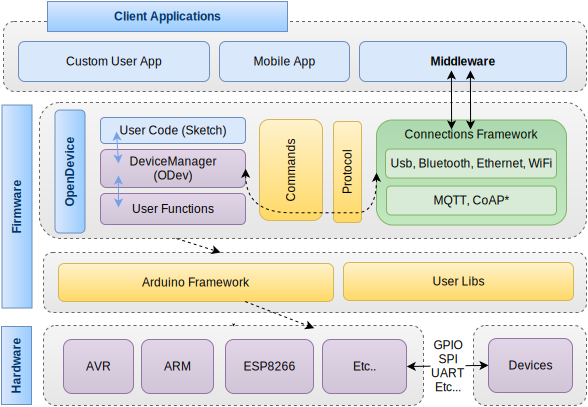
\includegraphics[width=1\linewidth]{Imagens/Cap_4/arquitetura-firmware}
\par\end{centering}
\caption{Arquitetura do Firmware\label{fig:ArquiteturaFirmware}}
\end{figure}


\subsection{Meios de comunicação suportados}

A tabela \ref{tab:FirmwareConexoes} apresenta as tecnologias de comunicação
que são suportadas, destacadas juntos com os modelos de comunicação.
Entende-se por modelo de comunicação a forma como o firmware irá operar,
se é no modo cliente ou no modo servidor.

\begin{table}[h]
\begin{centering}
\begin{tabular}{|c|c|c|}
\hline 
Tipo & Cliente & Servidor\tabularnewline
\hline 
\hline 
Usb & Não & Sim\tabularnewline
\hline 
Bluetooth & Não & Sim\tabularnewline
\hline 
Ethernet & Sim & Sim\tabularnewline
\hline 
Wi-Fi & Sim & Sim\tabularnewline
\hline 
\end{tabular}
\par\end{centering}
\caption{Comunicação suportada pelo firmware\label{tab:FirmwareConexoes}}

\end{table}


\subsection{Gerenciamento de conexões\label{subsec:FirmwareGerenciamentoConn}}

O bloco denominado ``Connections Framework'', trata-se de adaptações
das bibliotecas disponibilizadas pelo Arduino (``User Libs'' e nativas)
para implementação das conexões, usando seus respectivos módulos módulos
(shields), permitindo assim a comunicação com o middleware e aplicações.
Por exemplo, o suporte a conexões Ethernet usando o módulo ENC28J60,
necessita de uma biblioteca específica que realiza a implementação
do protocolo TCP/IP via software, já o modulo(shield) Ethernet baseado
no chip W5100 é suportado nativamente pelo framework do Arduino e
OpenDevice. O Arduino disponibiliza uma API base para implementação
das conexões Ethernet e Wi-Fi. Módulos (shields) que implementem essa
API estariam compatíveis automaticamente com o OpenDevice. 

As conexões USB e Bluetooth, são comunicações seriais, acessíveis
através de portas UART, referenciadas geralmente pelas variáveis
\emph{Serial}, \emph{Serial1}, etc. E que têm como implementação base
a classe \emph{Stream}(do Arduino). Outras tecnologias de conexão,
que se baseiem nos mecanismos apresentados acima serão automaticamente
suportados, ou necessitariam de pequenos ajustes. 

As tecnologias implementadas estão listadas na tabela \ref{tab:FirmwareConexoes}
e mais adiante na seção de hardwares testados (\ref{par:Hardwares-Testados});

\subsection{Gerenciamento dos dispositivos}

No firmware é realizado o mapeamento dos dispositivos e seus respectivos
IDs para os pinos do microcontrolador. Ele interpreta os comandos
enviados pelas aplicações e as transforma em ações. Um exemplo de
mapeamento dos dispositivos é demonstrado da listagem \ref{alg:firmware1},
onde é feita a configuração de forma estática, adicionando atuadores
e sensores. As classes que abstraem os dispositivos existem, e são
baseados na classe Device, e conta com um atributo do tipo \emph{booleano}
chamado \textquotedbl{}sensor\textquotedbl{}, para identificar se
é um atuador ou sensor. 

\begin{algorithm}[H]
\inputencoding{latin9}\begin{lstlisting}[language={C++}]
#include <OpenDevice.h>
// Mapeamento dos Dispositivos
void setup(){
	ODev.name("ODev-Thing1");
    ODev.addCommand("alertMode", alertMode);
    ODev.addDevice(5, Device::DIGITAL); // ID:1
    ODev.addSensor(3, Device::DIGITAL); // ID:2 
    ODev.addSensor(RFIDSensor(10,9)); // ID:1
    ODev.begin();
}

void loop(){
  ODev.loop();
}
// Comando de Usuario
void alertMode(){
  ODev.debug(ODev.readString());
  int count = ODev.readInt();
  // ....
}
\end{lstlisting}
\inputencoding{utf8}
\caption{Exemplo de configuração do firmware\label{alg:firmware1}}
\end{algorithm}


\subsubsection{Dispositivos suportados}

A tabela \ref{tab:FirmwareDevices}, apresenta a lista de dispositivos
suportados nativamente. A extensão de dispositivos permite a inclusão
e suporte de novos dispositivos, sendo apresentado com mais detalhes
na seção \ref{subsec:FirmwareExtensibilidade}.

\begin{table}[h]
\begin{centering}
\begin{tabular}{|c|c|c|}
\hline 
Nome & Tipo & Biblioteca Extra\tabularnewline
\hline 
\hline 
Genérico Digital (1 pino) & Atuador / Sensor & Não\tabularnewline
\hline 
Genérico Analógico (1 pino) & Atuador / Sensor & Não\tabularnewline
\hline 
RFID (MFRC522) & Sensor & Sim\tabularnewline
\hline 
Servo Motor & Atuador & Não\tabularnewline
\hline 
Temperatura (LM35) & Sensor & Não\tabularnewline
\hline 
Infra-Vermelho (Emissor) & Atuador & Sim\tabularnewline
\hline 
Infra-Vermelho (Receptor) & Sensor & Sim\tabularnewline
\hline 
\end{tabular}
\par\end{centering}
\caption{Dispositivos suportados nativamente\label{tab:FirmwareDevices}}
\end{table}


\subsection{Comandos de Usuário}

Os desenvolvedores podem criar novos comandos, estendendo o protocolo
ou usando os recursos de comandos do usuário (\emph{User Functions},
na figura \ref{fig:ArquiteturaFirmware}). Esse recurso permite criar
novos comandos e vinculá-los à funções definidas pelo próprio usuários.
A listagem \ref{alg:firmware1}, apresenta um exemplo desse recurso.
Os comandos são criados usando a função ``\inputencoding{latin9}\lstinline!ODev.addCommand!\inputencoding{utf8}'',
definindo o nome e a função que será executada ao receber esse comando.
No lado da aplicação (Java), esse comando é executado através do método:
``\inputencoding{latin9}\lstinline!sendCommand("alertMode","Your String", 5)!\inputencoding{utf8}''.
Observe que também é possível passar parâmetros para a função, e no
lado do firmware os parâmetros podem ser recuperados usando as funções
``\inputencoding{latin9}\lstinline!ODev.read*()!\inputencoding{utf8}''.

\subsection{Mecanismos de leitura de sensores\label{subsec:FirmwareLeituraSensores}}

O mecanismo de leitura adotado, também é um sistema baseado em eventos,
ou seja, as aplicações não precisam realizar consultas para obter
os valores dos sensores. Quando houver alguma alteração no valor do
sensor, automaticamente o firmware envia o valor atualizado para as
aplicações. Internamente, o mecanismo de leitura opera de dois modos:
síncrono e assíncrono, que serão apresentados a seguir.

\subsubsection{Modo Síncrono (Polling)}

O mecanismo síncrono ou ``polling'', é o mecanismo ativo por padrão,
e por ser uma implementação mais simples, pode ser utilizado em qualquer
microcontrolador, porém existem algumas limitações. Por se tratar
de um mecanismo onde é preciso realizar uma leitura de todos os sensores(pinos)
configurados, e comparar o valor lido com o valor atual, algum tempo
será perdido lendo sensores que não alteraram seu valor, e consumindo
recursos desnecessários CPU, que poderia estar desempenhando outras
atividades. Dependendo do tempo da leitura dos sensores, alguma informação
importante pode ser perdida. A leitura de pinos digitais e analógica
é bem rápida, a leitura de um pino analógico por exemplo, demora cerca
de 100 microssegundos~(0.0001 s), em um processador AVR 8-bits\footnote{https://www.arduino.cc/en/Reference/analogRead}.

\subsubsection{Modo Assíncrono (Interrupções)}

As interrupções são sinais enviados para o microcontrolador com eventos
que precisam de imediata atenção. A interrupção permite que o processador
interrompa a tarefa atual , salve seu contexto, e execute um rotina
especial de interrupção, conforme na figura \ref{fig:interrupcoes}.
Quando um dispositivo precisa de atenção ele envia um sinal para o
processador que desloca a execução para rotina de interrupção (ISR).
O suporte a interrupção externas (mudança nos pinos de I/O), depende
do microcontrolador, alguns suportam interrupções em todos os pinos
e outros suportam interrupções apenas em alguns pinos predefinidos.
Para citar exemplos, o Arduino DUE (SAM3X8E ARM) possui suporte a
interrupções externas em todos os pinos, já o Arduino Uno (e similares
com chip ATmega328p) suporta interrupções externas apenas nos pinos
2 e 3. 

Para lidar com as limitações encontradas, o firmware utiliza uma biblioteca\footnote{https://github.com/GreyGnome/EnableInterrupt}
que permite habilitar a associação de rotinas de interrupções individuais
para todos os pinos do microcontrolador, fazendo o gerenciamento do
estado dos pinos. Algumas limitações também são encontradas nessa
alternativa. O tempo de interrupção pode sofrer atrasos na ordem de
alguns micro-segundos para pinos que não suportem nativamente as interrupções
externas. Dependendo da aplicação isso pode ser relevante. Uma análise
realizada dos tempos de tratamento das interrupções, nessa implementação,
é apresentada em \cite{key-isr}.

Para habilitar o suporte a interrupções em um sensor é preciso habilitar
o recurso nas configurações gerais e ativar os sensores que serão
lidos com base nas interrupções. Com base no exemplo da listagem \ref{alg:interrupcoes},
quando ocorre alguma interrupção nos sensores configurados, os valores
deles são lidos pela rotina \emph{``OpenDeviceClass::onInterruptReceived()}'',
e marcados para sincronização, que irá ocorrer no ciclo de ``loop''.
Um ponto importante é que os dados não podem ser enviados na rotina
de interrupção, pois ela deve ocorrer o mais rápido possível, evitando
problemas na leitura de outras interrupções e podem ocasionar conflitos
com as interrupções de leituras das portas seriais. Detalhes de execução
desse fluxo serão apresentados na seção \ref{subsec:LeituraSensores}.

\begin{algorithm}[H]
\inputencoding{latin9}\begin{lstlisting}[language={C++}]
#include <EnableInterrupt.h>
#include <OpenDevice.h>

void setup() {
  // Modo 1
  ODev.addSensor(3, Device::DIGITAL)->enableInterrupt(CHANGE); // ID:1
  // Modo 2
  Device *s2 = ODev.addSensor(4, Device::DIGITAL); // ID:2
  *s2->enableInterrupt(CHANGE);
  
  ODev.begin();
}

void loop() {
  ODev.loop();
}
\end{lstlisting}
\inputencoding{utf8}
\caption{Leitura usando interrupções (Arduino/C++) \label{alg:interrupcoes}}
\end{algorithm}

\begin{figure}
\begin{centering}
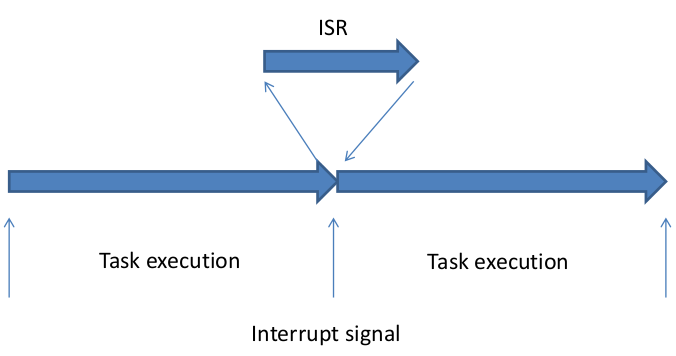
\includegraphics[width=1\linewidth]{Imagens/Cap_4/firmware_interrupcao}
\par\end{centering}
\caption{Execução de uma interrupção\label{fig:interrupcoes}}
\end{figure}


\subsection{Configuração dinâmica e parametrizações\label{subsec:ConfiguracaoDinamica}}

O firmware tenta detectar o hardware e as bibliotecas utilizadas e
realizar as parametrizações necessárias, necessitando o mínimo de
configurações possíveis. Um exemplo da técnica é apresentado na listagem
\ref{alg:firmware2}, onde a implementação da Ethernet é alterada
apenas escolhendo o \emph{``include''} correspondente, sem necessidade
de alterações no código. As duas implementações são totalmente diferentes,
porém essas diferenças são abstraídas pelo firmware, permitindo que
o desenvolvedor foque na lógica do sistema.

Algumas parametrizações e valores padrão, como velocidade, portas,
tamanhos dos \emph{buffers} de recepção de dados, podem ser ajustados
no arquivo: ``config.h'', bem como é possível habilitar o modo de
depuração (debug), para auxiliar na detecção de algum erro que esteja
ocorrendo. As informações de depuração podem ser direcionadas para
a conexão atual ou para uma porta serial do microcontrolador.

\begin{algorithm}[H]
\inputencoding{latin9}\begin{lstlisting}[language={C++}]
//#include <UIPEthernet.h> // ENC28J60
#include <Ethernet.h>
#include <OpenDevice.h>

void setup(){
  ODev.addDevice(13, Device::DIGITAL);
  ODev.begin();
}

void loop(){
  ODev.loop();
}
\end{lstlisting}
\inputencoding{utf8}
\caption{Exemplo de configuração do firmware\label{alg:firmware2}}
\end{algorithm}


\subsection{Monitoramento}

O sistema de monitoramento permite informar às aplicações a utilização
da memória RAM e EPROM do microcontrolador e monitorar os estados
das conexões, utilizando um mecanismo de Keep-Alive / Heartbeat. Em
algumas situações pode ocorrer que algumas das partes da comunicação
fique fora de sincronia, devido a problemas no link, falhas de software
ou hardware. Esse estado é geralmente chamado conexão semi-aberta
(half-open connection). É importante que o lado da conexão que está
funcionando corretamente seja notificado ou detecte a falha da outra
ponta, e tente uma reconexão ou fecha a conexão semi-aberta. Mesmo
existindo mecanismos similares em alguns protocolos como o TCP/IP,
ele pode não ser ideal para alguns tipos de aplicações, pois em média
ele é executado em um intervalo de duas horas e não permite ajustes
a nível de aplicações, necessitando de ajustes no sistema operacional\cite{key-keepa}.
Por outro lado, outras conexões (ex.: USB) não suportaram este mecanismo.
Para contornar esses problemas, o recurso de Keep-Alive / Heartbeat
foi implementado no firmware. Quando é habilitado o suporte ao protocolo
MQTT, o mecanismo de Keep-Alive do próprio protocolo são utilizados.

Este mecanismo é implementado através do envio de comando do tipo
PING, em um intervalo ajustável e aguardando seu retorno através do
comando do tipo PING\_RESPONSE, podendo ser habilitado e desabilitado
conforme a necessidade. Ao detectar uma falha ou estouro do tempo
determinado (time-out), a aplicação ou middleware decide o que fazer
com a conexão em estado inválido, se tenta uma reconexão ou finaliza
a conexão, liberando os recursos alocados.


\subsection{Extensibilidade\label{subsec:FirmwareExtensibilidade}}

O firmware é projetado como uma biblioteca, permitindo aos desenvolvedores
facilmente customizar e criar seu próprio firmware através da inclusão
do código de usuário (Sketch, vide figura \ref{fig:ArquiteturaFirmware}).
O mecanismo de conexões (Connections Framework) também é flexível,
permitindo plugar novas conexões facilmente, através da extensão da
classe \emph{DeviceConnection}, ou através do mecanismo de ``Custom
Connections'', que permite a criação de novas conexões, sobrescrevendo
métodos predefinidos usando apenas arquivos de cabeçalho (.h). Mais
detalhes serão apresentados a seguir.

A classe Device pode ser estendida para dar suporte a dispositivos
(sensores ou atuadores) mais complexos, que utilizem mais de um pino
ou trabalhem com um protocolo específico (ex.: SPI, OneWire). Um exemplo
de especialização desta classe é realizado pele classe \emph{RFIDSensor},
disponível nas bibliotecas do firmware, que permite a integração de
um sensor RFID de proximidade (baseado no chip MFRC522). A inclusão
de novos dispositivos, é realizada estendendo a classe Device e implementando
os métodos ``setValue'' e ``hasChanged''. 

Outro método de inclusão de novos dispositivos, mais especificamente
sensores, permite a integração com sensores mais complexos (que utilizem
um protocolo específico), de uma forma simplificada e sem a necessidade
de estender a classe Device, facilitando assim a integração e testes.
A listagem \ref{alg:firmware-newsenor} apresenta um exemplo deste
recurso, onde a leitura do sensor é implementada por um método definido
pelo usuário no programa principal (Sketch), onde o método deve retornar
a leitura do sensor. O firmware é responsável por executar esse método
e verificar se houve alguma mudança no valor do sensor, caso exista
alguma alteração, as aplicações são notificadas.

\begin{algorithm}[H]
\inputencoding{latin9}\begin{lstlisting}[language={C++}]
void setup(){
    ODev.addSensor(readRfid); // ID:1
    // ... sensor setup ...
    ODev.begin();
}

unsigned long readRfid(){
  // sensor logic
}
\end{lstlisting}
\inputencoding{utf8}
\caption{Suporte a novos sensores\label{alg:firmware-newsenor}}
\end{algorithm}


\subsubsection{Mecanismo ``Custom Connections''}

Nativamente o \emph{firmware} suporta qualquer conexão que estenda
a classe \emph{Stream} (do Arduino). Caso seja necessário a inclusão
de outro mecanismo de comunicação, onde a biblioteca projetada para
o mesmo não implemente a classe Stream, um ``adaptador'' pode ser
criado para essa conexão. Exemplos dessa implementação são encontrados
no próprio firmware (arquivo: EthernetServerConnection.h) e a estrutura
básica é apresentada na listagem \ref{alg:firmware-custconn}. A vantagem
é que não é necessária a criação de classes (C++), necessitando apenas
de um arquivo de cabeçalho (.h). Ao realizar a inclusão deste cabeçalho
no programa, o firmware automaticamente detecta que deve ser usado
essa conexão e realiza as chamadas dos métodos implementados. É importante
que a classe retornada pelo método ``\_loop()'', seja uma instância
e estenda a classe ``Stream'' para que o mecanismo funcione. 

\begin{algorithm}[H]
\inputencoding{latin9}\begin{lstlisting}[language={C++}]
#define USING_CUSTOM_CONNECTION 1
#define CUSTOM_CONNECTION_CLASS YourClassExtendStream

void custom_connection_begin(){
  
}

CUSTOM_CONNECTION_CLASS custom_connection_loop(DeviceConnection *conn){
  return // return instance of YourClassExtendStream;
}

\end{lstlisting}
\inputencoding{utf8}
\caption{Exemplo do mecanismo ``Custom Connections'' \label{alg:firmware-custconn}}
\end{algorithm}


\section{Fluxo de Mensagens\label{subsec:FluxoMensagens}}

Nesta seção abordamos os principais fluxos de execução, encontrados
no firmware, middleware e aplicações, auxiliando a entender o processo
interno de execução e quais componentes são utilizados em cada etapa.

\subsection{Envio de Comandos\label{subsec:FluxoEnvioComandos}}

A figura \ref{fig:seq_command_send}, apresenta o fluxo de envio de
comandos entre uma aplicação, que se comunica diretamente com os dispositivos
(firmware). A primeira etapa inicia com a abstração do dispositivo
e a execução do seu método ``on'' ou ``setValue'' (ex.: led.on()).
Esse método gera um evento que é capturado pelo framework (fluxo 1),
através da classe \emph{DeviceManager}, que cria o comando apropriado,
no caso o \emph{DeviceCommand}, e inicializa com as informações do
ID do dispositivo, tipo (ANALOG ou Digital) e valor e repassa para
o CommandDelivery (fluxo 1.2), que cuida do envio para as conexões
de saída de modo assíncrono, usando a \emph{SendTask}. As mensagens
são serializadas para o formato do protocolo (\ref{subsec:Protocolo})
do OpenDevice usando o \emph{MessageSerializer}. Cada comando enviado,
recebe um ID (TrackingID), que é gerenciado pelo CommandDelivery,
e é usado para fazer o mapeamento dos comandos enviados e comandos
recebidos (fluxo 2 e 3). O ID do comando é gerado de forma sequencial,
até um limite estabelecido pelo protocolo, depois é reiniciado a contagem.
A SendTask, é registrada para receber os eventos das conexões. Quando
a resposta é recebida pela conexão, o método ``onMessageReceived''
(fluxo 3) é executado, e a resposta é mapeada para o comando enviado.

\begin{figure}[h]
\begin{centering}
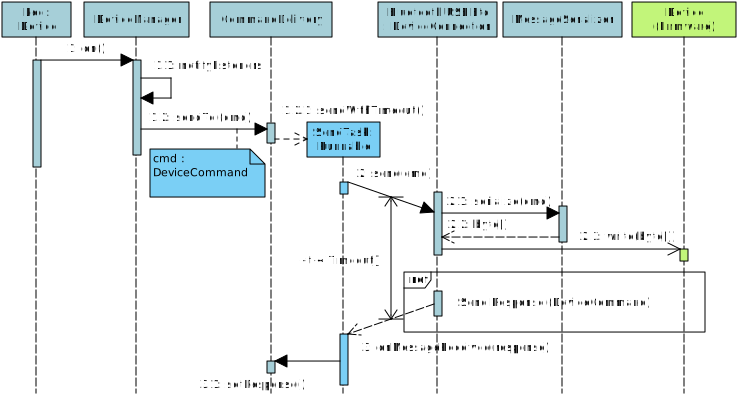
\includegraphics[width=1\linewidth]{Imagens/Cap_4/seq_command_send}
\par\end{centering}
\caption{Envio de Comandos\label{fig:seq_command_send}}
\end{figure}


\subsection{Processamento dos Comandos (Dispositivo)}

A figura \ref{fig:seq_firmware_read}, demonstra o fluxo de execução
do firmware, para realizar a leitura dos comandos das aplicações (ou
do middleware), transforma-lo em ações reais.

Os comandos recebidos são tratados por uma implementação da classe
\emph{Stream} (fluxo 1), que pode ser uma implementação nativa do
Arduino, como a \emph{Serial} ou \emph{EthernetClient}, ou uma implementação
disponibilizada por uma biblioteca de terceiros, que implementa outra
tecnologia de comunicação. Geralmente esses dados são armazenados
em um buffer, de software ou de hardware, e serão lidos no ciclo de
``loop'' do programa principal, através da chamada do ``checkDataAvailable''
(fluxo 2), que ao identificar o final da mensagem especificado no
protocolo, faz a desserialização através do método ``parseCommand''
( fluxo 2.3), e repassa para a classe principal da biblioteca do OpenDevice
(fluxo 2.4), que verifica que tipo de comando foi recebido e faz o
tratamento adequado. Caso a mensagem recebida (fluxo 2.4), seja um
\emph{DeviceCommand} (Ex.: Analogic ou Digital), o dispositivo relacionado
é localizado através do ``DeviceID'', e em seguida seu valor é alterado
(fluxo 3), conforme o valor recebido pelo comando. Em seguida a implementação
do Device determina como será o tratamento para o valor recebido.
Por exemplo, se o dispositivo for um dispositivo do tipo DIGITAL,
a implementação chama o método ``digitalWrite'' da API do Arduino,
caso seja um Device do tipo ANALOG, a implementação chama o método
``analogWrite''.

Quando um comando é recebido com sucesso e o dispositivo relacionado
é encontrado, uma resposta é enviada para a aplicação (fluxo 4.1.1),
informando o estados da execução. Essa resposta é encapsulada através
da classe \emph{ResponseCommand}, podendo ter vários status, conforme
a tabela \ref{tab:CommandStatusResp}, na seção referente ao protocolo
(\ref{subsec:Protocolo}).

\begin{figure}[h]
\begin{centering}
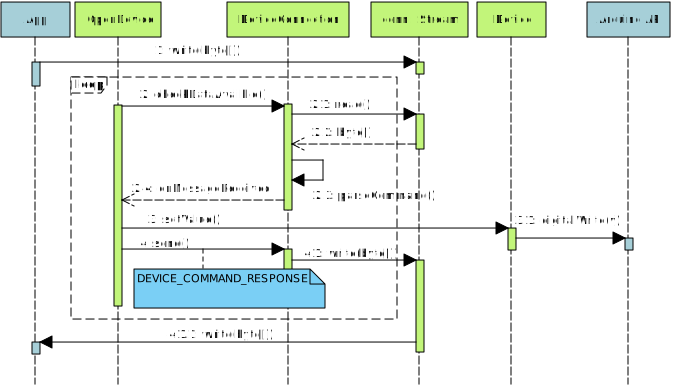
\includegraphics[width=1\linewidth]{Imagens/Cap_4/seq_firmware_read}
\par\end{centering}
\caption{Processamento dos Comandos\label{fig:seq_firmware_read}}
\end{figure}


\subsection{Recebimento de Comandos}

O diagrama de sequência apresentado na figura \ref{fig:seq_send_response},
trata-se da continuação do fluxo, quando o dispositivo (firmware)
devolve a resposta com o status da execução do comando para a aplicação
ou middleware. O componente que fará a leitura dos dados brutos, depende
da implementação da conexão. No exemplo da figura, foi utilizando
um \emph{StreamReader}, mais especificamente \emph{CommandStreamReader},
que é a implementação base para lidar com as conexões implementados
no módulo \noun{connection-stream} (USB e Bluetooth por exemplo).
Essa implementação em específico, utiliza uma ``thread'' para leitura
dos dados de cada conexão, e ao identificar o recebimento do pacote
completo, ele notifica a conexão (fluxo 1.3), que por sua vez notifica
os componentes interessados (fluxos 2 e 3).

Quando se trata de uma resposta de um comando, por exemplo DeviceCommand,
a SendTask, criada e gerenciada pelo CommandDelivery, é notificada
e atualiza o status do comando que foi enviado, com base do ID do
comando (TrackingID) e faz a liberação (remove a trava) do comando.

Caso não seja uma resposta de um comando, por exemplo a leitura de
um sensor, o CommandDelivery não é utilizado . O responsável por tratar
esse comando é o DeviceManager, como será visto na seção seguinte
(\ref{subsec:LeituraSensores}).

\begin{figure}[h]
\begin{centering}
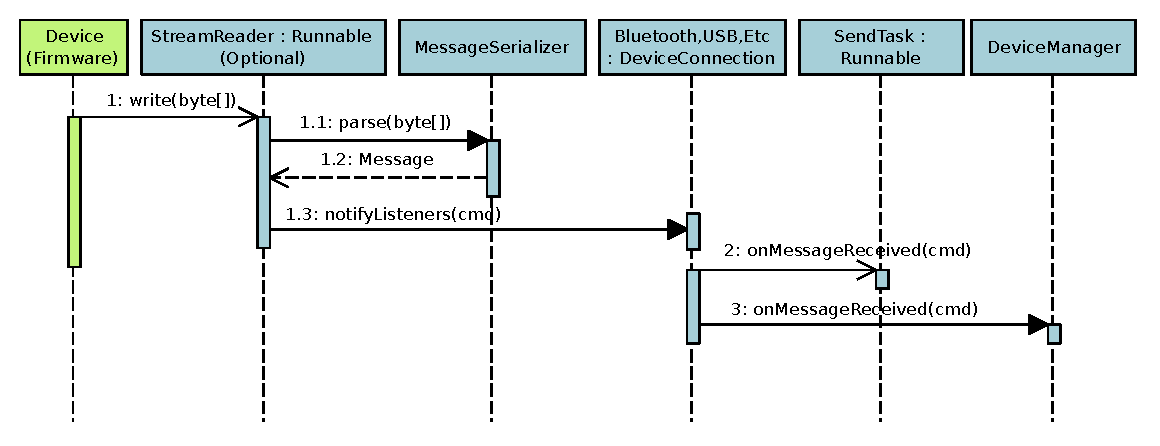
\includegraphics[width=1\linewidth]{Imagens/Cap_4/seq_send_response}
\par\end{centering}
\caption{Recebimento de Comandos\label{fig:seq_send_response}}
\end{figure}


\subsection{Leitura de Sensores\label{subsec:LeituraSensores}}

O fluxo da leitura de sensores, apresentados nas figuras \ref{fig:seq_firmware_read_poll}
e \ref{fig:seq_firmware_read_interrupt}, trata-se também de um fluxo
de recebimento de comandos, é similar ao da figura \ref{fig:seq_send_response}.
Como abordamos na seção \ref{subsec:FirmwareLeituraSensores}, o sistema
de leitura de sensores é implementado de dois modos: síncrono (polling)
e assíncrono (interrupções). O modo utilizado depende do suporte que
o \emph{hardware.} Como exemplo, utilizamos um microcontrolador AVR~8Bits~(ex.:
Arduino), executando o firmware, e enviando os dados dos sensores
para a aplicação (ou middleware).

\subsubsection{Leitura Síncrona (Polling)}

No modo síncrono, a leitura dos sensores é feito no ``loop'' principal,
e é realizada pela classe \emph{OpenDevice}, através do método ``checkSensorsStatus()''
(fluxo 1). Neste método todos os sensores serão lidos de forma sequencial,
através do método ``hasChanged()'' da classe Device. Ao executar
esse método o valor do dispositivo é atualizado, e caso tenha sofrido
alguma alteração (fluxo 1.1.2), um comando (\emph{DeviceCommand})
com o ID do dispositivo e valor lido é enviado para ao conexão (fluxo
1.2), que cuida de serializar e enviar os dados para a aplicação.

\begin{figure}[h]
\begin{centering}
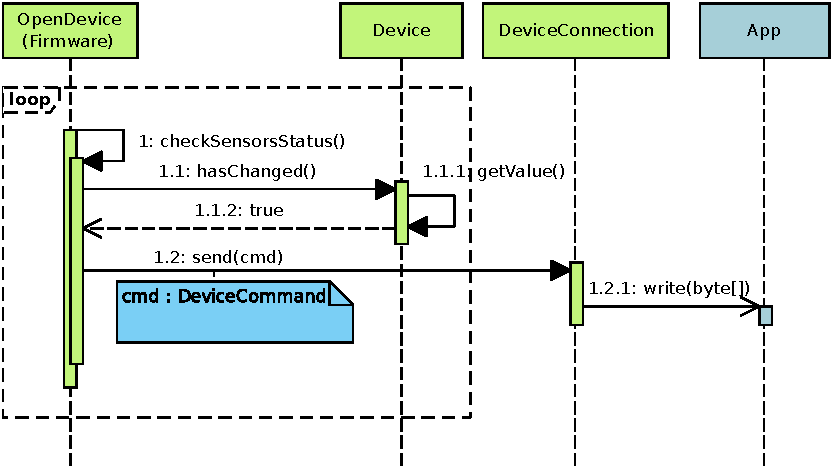
\includegraphics[width=1\linewidth]{Imagens/Cap_4/seq_firmware_read_poll}
\par\end{centering}
\caption{Leitura de Sensores no modo Polling\label{fig:seq_firmware_read_poll}}
\end{figure}


\subsubsection{Leitura Assíncrona (Interrupções)}

O método de leitura assíncrona, apresentado na figura \ref{fig:seq_firmware_read_interrupt},
é realizado através de interrupções, como mencionamos na seção \ref{subsec:FirmwareLeituraSensores}.
Quando habilitado o suporte a interrupções, a classe OpenDevice é
registrada para receber as interrupções através do método ``onInterruptReceived()''.
Neste método o dispositivo correspondente ao pino que sofreu a interrupção
é localizado, e seu valor é atualizado. Os dispositivos que sofrerem
alterações nos seus valores durante a interrupção, são marcados para
sincronização (fluxo 1.2), que irá ocorrer na próxima execução do
“loop” principal do programa. Similar à leitura síncrona, o método
``checkSensorsStatus()'' é chamada no ``loop'', porém neste caso
não é feito nenhuma leitura dos pinos, apenas o envios das informações
para dos dispositivos que sofreram alterações para a aplicação (fluxo
1.2 e 2.1). A vantagem neste caso é que enquanto estão sendo enviadas
as informações para aplicação, caso algum dispositivo tenha seu valor
alterado, a interrupção cuida de deslocar o fluxo de execução, salvar
esse valor e retornar para a serialização dos dados. Na implementação
no modo síncrona (polling), esse valor seria perdido.

\begin{figure}[h]
\begin{centering}
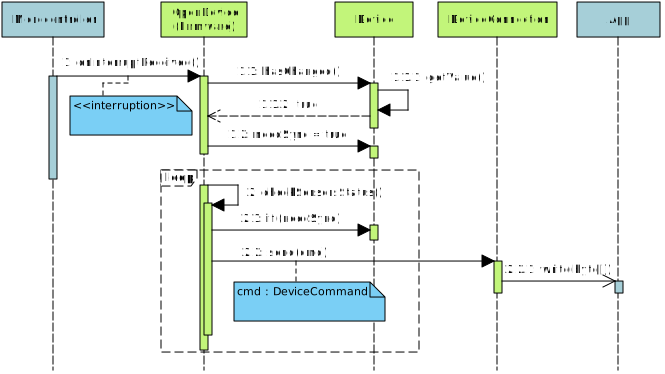
\includegraphics[width=1\linewidth]{Imagens/Cap_4/seq_firmware_read_interrupt}
\par\end{centering}
\caption{Leitura de Sensores usando Interrupções\label{fig:seq_firmware_read_interrupt}}
\end{figure}


\subsection{Envio de Comandos (Aplicação - Middleware - Dispositivo)}

A figura \ref{fig:seq_send_ws}, apresenta o fluxo de execução de
um comando enviado por uma aplicação cliente (WebApp) para os dispositivos,
através do middleware. O framework trabalha com dois conceitos de
conexões: (1) conexões de entrada, ou seja, os servidores e (2) conexões
de saída, geralmente as conexões com os dispositivos físicos. O componente
representado em ``WSServerConnection'', é um servidor WebSocket
disponibilizado pelo módulo \noun{rest-ws-server, }que atua como uma
conexão de entrada. A aplicação web no exemplo, está utilizando a
biblioteca \noun{opendevice-js}, uma das implementações de cliente
usando WebSocket, permitindo a conexão de forma simples com o servidor,
e oferecendo a abstração dos dispositivos para a camada Web.

Ao alterar o valor de algum dispositivo na camada Web, que pode ser
através dos métodos nos objetos JavaScript (fluxo 2), ou através de
métodos disponibilizados no \noun{opendevice-js}, um comando é enviado
via WebSocket para o Middleware (fluxo 2.1). A representação da conexão
com o cliente ``WSResource'' recebe o comando (fluxo 2.1.1) e notifica
para o DeviceManager (fluxos 2.1.2 e 2.1.2.1), que faz a atualização
do dispositivo relacionado ao comando recebido, salva no histórico
de alterações, e repassa o comando para os dispositivos físicos através
das conexões de saída. O procedimento de envio, representado na imagem
pelo bloco ``Ref: Send Command'', é o mesmo procedimento realizado
no fluxo apresentado na seção Envio de Comandos (\ref{subsec:FluxoEnvioComandos}).

O recebimento da resposta do dispositivo físico (fluxo 3), é redirecionado
para a conexão de origem (WSResource). O redirecionamento é feito
baseado na identificação da conexão (UUID), que é gerado no momento
de sua criação (fluxo 1.1.1), e o mesmo é associado ao comando quando
ele é enviado ou recebido, sendo então possível enviar a resposta
para o cliente correto. Deste modo é possível permitir que múltiplas
aplicações acessem o mesmo dispositivo, contornando as limitações
do USB e Bluetooth que permitem apenas um cliente, ou mesmo de conexões
Ethernet ou Wi-Fi, que dependendo do hardware, podem suportar apenas
um cliente ou um número limitado.

\begin{figure}[h]
\begin{centering}
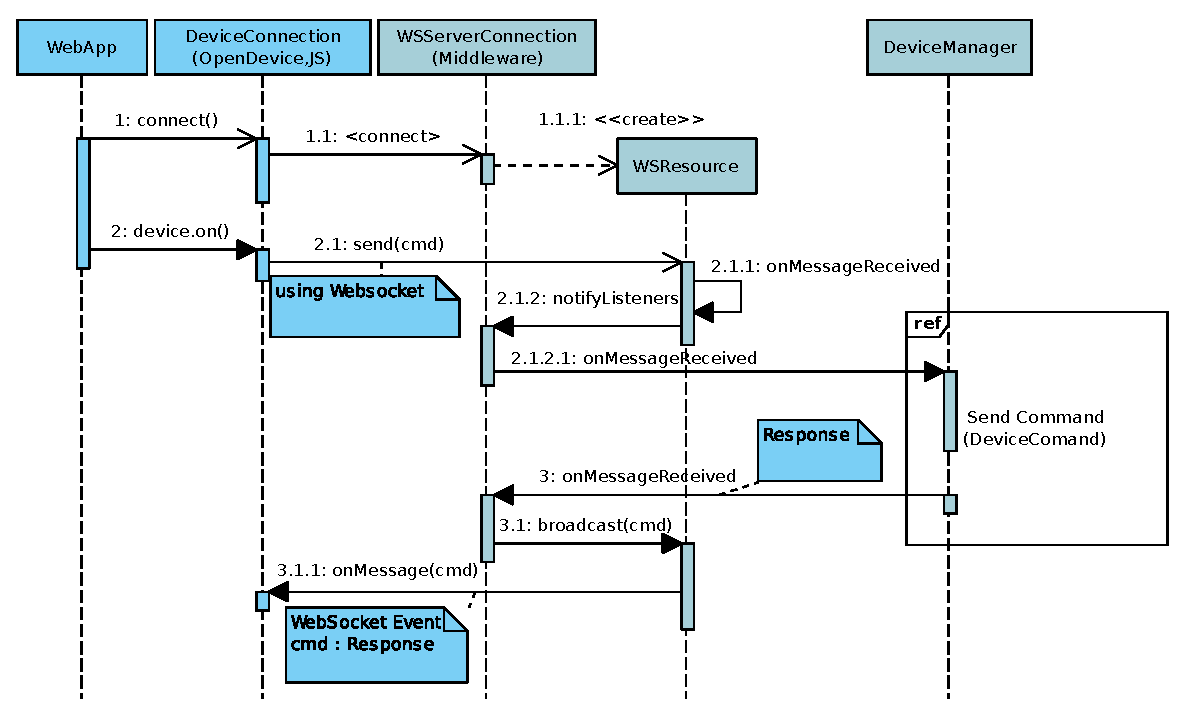
\includegraphics[width=1\linewidth]{Imagens/Cap_4/seq_send_ws}
\par\end{centering}
\caption{Envio de comandos\label{fig:seq_send_ws}}
\end{figure}


\section{Protocolo\label{subsec:Protocolo}}

Esta seção apresenta o protocolo do OpenDevice. As principais características
do protocolo é que ele foi projetado para ser um protocolo aberto,
leve, simples, de fácil implementação, legível para humanos e voltado
para dispositivos com restrições de memória e processamento, como
por exemplo, microcontroladores (AVR 8-bits, 2Kb de RAM).

O protocolo é baseado em ASCII (assim como o HTTP), orientado a mensagens/comandos
e assíncrono. Surgiu de algumas influências do protocolo MIDI (formato
usado para comunicação com instrumentos musicais) e do protocolo REST
na sua estrutura básica. 

O protocolo foi projetado para permitir a abstração, controle de dispositivos
(atuadores), realizar a leitura de sensores e ser de fácil extensão,
mas não limitado a isto. Ele pode ser utilizado em conjunto com outros
protocolos, como WebSocket e MQTT, e com outras tecnologias de comunicação,
como: USB, Bluetooth, Ethernet, Wi-Fi, etc. 


\subsection{Formato da Mensagem}

Os comandos do OpenDevice possuem um ``cabeçalho'' fixo, contento
o tipo do comando (\emph{CommandType}) e o ID do comando, em seguida,
o bloco \emph{``Command Extension}'', que varia de acordo com o
tipo de comando. 

\begin{figure}[H]
\begin{centering}
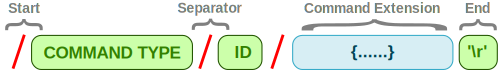
\includegraphics[width=0.8\linewidth]{Imagens/Cap_4/protocol_spec}
\par\end{centering}
\caption{Formato do protocolo OpenDevice \label{fig:protocol_spec}}
\end{figure}

\begin{itemize}
\item O \textbf{tipo do comando} define a estrutura do bloco ``\emph{Command
Extension}''. Os tipos suportados estão definidos na tabela \ref{tab:CommandType}. 
\item O \textbf{ID} do comando é numérico, sequencial e gerenciado pela
aplicação cliente. Ele serve para a aplicação identificar o retorno(resposta)
de algum comando enviado. Quando atinge seu valor máximo a contagem
reinicia.
\item Os blocos do comando são separados através do caractere ``/''.
\item O comando finaliza com o terminador ``\textbackslash{}r'' (Carriage
return).
\end{itemize}
\noun{Observação:} Na implementação atual do firmware, tanto o ``tipo
do comando'' quanto o ``id'', são armazenados em varáveis de 8bits
(uint8\_t / byte), limitando a valores na faixa de 0 a 255. Porém,
os mesmos são parametrizados podendo escolher outros tipos como: uint16\_t
ou uint32\_t.

\subsubsection{Convenções e pontos em aberto}

Algumas convenções foram adotadas para determinar observações, e destacar
pontos em aberto. Caso o texto apresente ``{[}{*}Numero{]}'', significa
que deve ser verificado as observações abaixo:
\begin{itemize}
\item Observação {[}{*}1{]}\noun{:} Na implementação atual do firmware,
o ``DeviceID'' é armazenado em uma variável de 8bits (byte), porém,
o tipo é parametrizável.
\item Observação {[}{*}2{]}\noun{: }Significa que o parâmetro ou tipo é
configurável. 
\item Observação {[}{*}3{]}\noun{:} Significa que a versão atual do firmware
não implementa o recurso.
\end{itemize}

\subsection{Tipos de Comandos}

A tabela \ref{tab:CommandType}, apresenta os tipos de comandos suportados.

\begin{table}[H]
\noindent\resizebox{\textwidth}{!}{
\begin{centering}
\begin{tabular}{|c|l|c|l|}
\hline 
Código & Tipo de Comando & Ref. & Formato\tabularnewline
\hline 
\hline 
1 & DIGITAL & \ref{subsec:DIGITAL} & {[}\#/\#{]}/\{DeviceID\}/\{value\}\tabularnewline
\hline 
2 & ANALOG & \ref{subsec:ANALOG} & {[}\#/\#{]}/\{DeviceID\}/\{value\}\tabularnewline
\hline 
3 & NUMERIC & \ref{subsec:NUMERIC} & {[}\#/\#{]}/\{DeviceID\}/\{value\}\tabularnewline
\hline 
4...9 & {[}Reservado{]} &  & –\tabularnewline
\hline 
10 & COMMAND\_RESPONSE & \ref{subsec:COMMAND_RESPONSE} & {[}\#/\#{]}/\{status\}/\{DeviceID?\}\tabularnewline
\hline 
11 & SET\_PROPERTY & \ref{subsec:SET_PROPERTY} & {[}\#/\#{]}/\{DeviceID\}/\{property\}/\{value\}\tabularnewline
\hline 
12 & GET\_PROPERTIES & \ref{subsec:GET_PROPERTIES} & {[}\#/\#{]}/\{DeviceID\}\tabularnewline
\hline 
13 & GET\_PROPERTIES\_RESPONSE & \ref{subsec:GET_PROPERTIES_RESPONSE} & {[}\#/\#{]}/\{DeviceID\}/{[}\{property1:value\},...,N{]}\tabularnewline
\hline 
14 & ACTION & \ref{subsec:ACTION} & {[}\#/\#{]}/\{DeviceID\}/\{action\}/{[}\{value1?\},...,\{valueN\}{]}\tabularnewline
\hline 
15 & GET\_ACTIONS & \ref{subsec:GET_ACTIONS} & {[}\#/\#{]}/\{DeviceID\}\tabularnewline
\hline 
16 & GET\_ACTIONS\_RESPONSE & \ref{subsec:GET_ACTIONS_RESPONSE} & {[}\#/\#{]}/\{DeviceID\}/{[}\{action1\},\{actionN\}{]}\tabularnewline
\hline 
16...19 & {[}Reservado{]} &  & –\tabularnewline
\hline 
20 & PING\_REQUEST & \ref{subsec:PING_REQUEST} & {[}\#/\#{]}{[}somente cabeçalho{]}\tabularnewline
\hline 
21 & PING\_RESPONSE & \ref{subsec:PING_RESPONSE} & {[}\#/\#{]}{[}somente cabeçalho{]}\tabularnewline
\hline 
22 & DISCOVERY\_REQUEST & \ref{subsec:DISCOVERY_REQUEST} & {[}\#/\#{]}{[}somente cabeçalho{]}\tabularnewline
\hline 
23 & DISCOVERY\_RESPONSE & \ref{subsec:DISCOVERY_RESPONSE} & {[}\#/\#{]}/\{name\}/\{port\}/\{deviceLength\}\tabularnewline
\hline 
24...29 & {[}Reservado{]} &  & –\tabularnewline
\hline 
30 & GET\_DEVICES & \ref{subsec:GET_DEVICES} & {[}\#/\#{]}/\{DeviceID?\}/\{value?\}\tabularnewline
\hline 
31 & GET\_DEVICES\_RESPONSE & \ref{subsec:GET_DEVICES_RESPONSE} & {[}\#/\#{]}/{[}\{DeviceInfo1\},\{DeviceInfoN?{]}\tabularnewline
\hline 
32 & DEVICE\_ADD & \ref{subsec:DEVICE_ADD} & {[}\#/\#{]}/\{DeviceInfo\}\tabularnewline
\hline 
33 & DEVICE\_DEL & \ref{subsec:DEVICE_DEL} & {[}\#/\#{]}/\{DeviceID?\}\tabularnewline
\hline 
41..100 & {[}Reservado{]} &  & \tabularnewline
\hline 
\end{tabular}
\par\end{centering}
}

\caption{Tipos de comandos do protocolo\label{tab:CommandType}}
\end{table}


\subsection{Comando: DIGITAL\label{subsec:DIGITAL}}

Este comando permite controlar os dispositivos digitais (atuadores)
ou notificar alguma mudança no estado/valor de um sensor. O comando
adiciona dois blocos adicionais: DeviceID e Value (Figura \ref{fig:protocol_cmd}). 

Ao enviar um comando para um dispositivo, por exemplo, ligar lâmpada,
o dispositivo deve retornar uma resposta (geralmente assíncrona),
com o status do comando. 

O formato da resposta é definida em \emph{``}\nameref{subsec:COMMAND_RESPONSE}'',
onde o ID da resposta será o mesmo ID do comando enviado.

\begin{figure}[H]
\begin{centering}
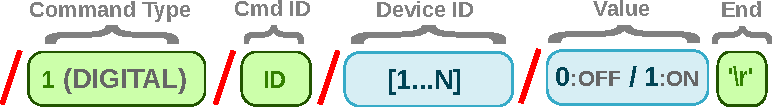
\includegraphics[width=0.8\linewidth]{Imagens/Cap_4/protocol_cmd_digital}
\par\end{centering}
\caption{Comando: DIGITAL\label{fig:protocol_cmd}}
\end{figure}

\begin{table}[H]
\begin{centering}
\begin{tabular}{|c|c|l|}
\hline 
Parâmetro & Tipo & Descrição\tabularnewline
\hline 
\hline 
DeviceID & byte {[}{*}1{]} & Identificador único que representa o dispositivo\tabularnewline
\hline 
Value & bool & 0 (Desligar / Desligado) ou 1 (Ligar / Ligado)\tabularnewline
\hline 
\end{tabular}
\par\end{centering}
\caption{Parâmetros - Comando: DIGITAL}
\end{table}


\subsection{Comando: ANALOG\label{subsec:ANALOG}}

Obedece o formado do ``\nameref{subsec:DIGITAL}'', mudando apenas
o tipo do comando, no caso 2, e o tipo de dado do bloco ``\emph{Value}'',
que pode aceitar valores do tipo \emph{``unsigned long}'', com tamanho
de 32 bits (4 bytes). 

Este comando pode ser utilizado tanto para sensores como para atuadores,
no caso de sensores, ele é utilizado para notificar um mudança de
estado (já que sensores são apenas para ``leitura'').

O formato da resposta é definida em \emph{``}\nameref{subsec:COMMAND_RESPONSE}'',
onde o ID da resposta será o mesmo ID do comando enviado.

\subsection{Comando: NUMERIC\label{subsec:NUMERIC}}

Obedece o formado do ``\nameref{subsec:ANALOG}''. Este comando
é utilizado em conjunto com os dispositivos (principalmente sensores)
do tipo \emph{NUMERIC}, que permitem o envio de informações repetidas.
Um exemplo, o sensor RFID, que gera um evento toda vez que uma etiqueta
é lida, mesmo sendo a mesma etiqueta.

\subsection{Reposta: COMMAND\_RESPONSE\label{subsec:COMMAND_RESPONSE}}

Representa a resposta de um determinado comando. As respostas são
associadas ao comando que a originou (requisição), através do atributo
``ID'' do cabeçalho fixo. Adicionalmente os comandos que referenciam
um dispositivo, na resposta, será incluído o mesmo ``DeviceID''
do comando da ``requisição''.

\begin{table}[H]
\begin{centering}
\begin{tabular}{|c|c|c|}
\hline 
\prth HEADER & \prtv Status & \prtv DeviceID\tabularnewline
\hline 
\end{tabular}
\par\end{centering}
\caption{Reposta: COMMAND\_RESPONSE}
\end{table}

\begin{table}[H]
\begin{centering}
\begin{tabular}{|c|c|l|}
\hline 
Parâmetro & Tipo & Descrição\tabularnewline
\hline 
\hline 
ID & byte {[}{*}2{]} & Mesmo ID enviado na requisição\tabularnewline
\hline 
Status & byte & Obedece aos valores da tabela: \ref{tab:CommandStatusResp}\tabularnewline
\hline 
DeviceID & byte {[}{*}1{]} (Opcional) & Mesmo ID enviado na requisição\tabularnewline
\hline 
\end{tabular}
\par\end{centering}
\caption{Parâmetros - Comando: COMMAND\_RESPONSE\label{tab:CommandStatusResp-1-1}}
\end{table}

\begin{table}[H]
\begin{centering}
\begin{tabular}{|c|c|}
\hline 
Status & Código\tabularnewline
\hline 
\hline 
SUCCESS & 200\tabularnewline
\hline 
NOT\_FOUND & 404\tabularnewline
\hline 
BAD\_REQUEST & 400\tabularnewline
\hline 
\textcolor{red}{UNAUTHORIZED {[}{*}3{]}} & 401\tabularnewline
\hline 
\textcolor{red}{FORBIDDEN {[}{*}3{]}} & 403\tabularnewline
\hline 
\textcolor{red}{PERMISSION\_DENIED {[}{*}3{]}} & 550\tabularnewline
\hline 
INTERNAL\_ERROR & 500\tabularnewline
\hline 
NOT\_IMPLEMENTED & 501\tabularnewline
\hline 
\end{tabular}
\par\end{centering}
\caption{Status da resposta do comando\label{tab:CommandStatusResp}}
\end{table}


\subsection{Comando: SET\_PROPERTY\label{subsec:SET_PROPERTY}}

Comando utilizado para atualizar alguma propriedade do dispositivo.
O formato da resposta é definido em \emph{``}\nameref{subsec:COMMAND_RESPONSE}''.

\begin{table}[H]
\begin{centering}
\begin{tabular}{|c|c|c|c|}
\hline 
\prth HEADER & \prtv DeviceID & \prtv property & \prtv value\tabularnewline
\hline 
\end{tabular}
\par\end{centering}
\caption{Comando: SET\_PROPERTY}
\end{table}

\begin{table}[H]
\begin{centering}
\begin{tabular}{|c|c|l|}
\hline 
Parâmetro & Tipo & Descrição\tabularnewline
\hline 
\hline 
DeviceID & byte {[}{*}1{]} & Identificador único que representa o dispositivo\tabularnewline
\hline 
property & String & Propriedade a ser alterada\tabularnewline
\hline 
value & String & Valor da propriedade\tabularnewline
\hline 
\end{tabular}
\par\end{centering}
\caption{Parâmetros: SET\_PROPERTY}
\end{table}


\subsection{Comando: GET\_PROPERTIES\label{subsec:GET_PROPERTIES}}

Comando utilizado para recuperar a lista de propriedades do dispositivo
e seus respectivos valores. O formato da resposta é definido em \emph{``}\nameref{subsec:GET_PROPERTIES_RESPONSE}''

\begin{table}[H]
\begin{centering}
\begin{tabular}{|c|c|}
\hline 
\prth HEADER & \prtv DeviceID\tabularnewline
\hline 
\end{tabular}
\par\end{centering}
\caption{Comando: GET\_PROPERTIES}
\end{table}

\begin{table}[H]
\begin{centering}
\begin{tabular}{|c|c|l|}
\hline 
Parâmetro & Tipo & Descrição\tabularnewline
\hline 
\hline 
DeviceID & byte {[}{*}1{]} & Identificador único que representa o dispositivo\tabularnewline
\hline 
\end{tabular}
\par\end{centering}
\caption{Parâmetros: GET\_PROPERTIES}
\end{table}


\subsection{Comando: GET\_PROPERTIES\_RESPONSE\label{subsec:GET_PROPERTIES_RESPONSE}}

Resposta do comando ``\emph{GET\_PROPERTIES}'', com a lista de propriedades
do dispositivo. A lista é retornada no formato de um Array, e os elementos
no formato: ``Propriedade:Valor''.

\begin{table}[H]
\begin{centering}
\begin{tabular}{|c|c|c|}
\hline 
\prth HEADER & \prtv DeviceID & \prtv{[}property:value,...,propertyN:value{]}\tabularnewline
\hline 
\end{tabular}
\par\end{centering}
\caption{Comando: GET\_PROPERTIES\_RESPONSE}
\end{table}

\begin{table}[H]
\begin{centering}
\begin{tabular}{|c|c|l|}
\hline 
Parâmetro & Tipo & Descrição\tabularnewline
\hline 
\hline 
DeviceID & byte {[}{*}1{]} & Identificador único que representa o dispositivo\tabularnewline
\hline 
property & String & Propriedade\tabularnewline
\hline 
value & String & Valor da propriedade\tabularnewline
\hline 
\end{tabular}
\par\end{centering}
\caption{Parâmetros: GET\_PROPERTIES\_RESPONSE}
\end{table}


\subsection{Comando: ACTION\label{subsec:ACTION}}

Comando usado para executar as ações definidas pelos dispositivos.
As ações podem receber uma lista de valores, que são especificados
em formato de Array. O formato da resposta é definido em \emph{``}\nameref{subsec:COMMAND_RESPONSE}''.

\begin{table}[H]
\begin{centering}
\begin{tabular}{|c|c|c|c|}
\hline 
\prth HEADER & \prtv DeviceID & \prtv action & \prtv{[}\{value1\},...,\{valueN\}{]}\tabularnewline
\hline 
\end{tabular}
\par\end{centering}
\caption{Comando: ACTION}
\end{table}

\begin{table}[H]
\begin{centering}
\begin{tabular}{|c|c|l|}
\hline 
Parâmetro & Tipo & Descrição\tabularnewline
\hline 
\hline 
DeviceID & byte {[}{*}1{]} & Identificador único que representa o dispositivo\tabularnewline
\hline 
action & String & Ação que deve ser executada\tabularnewline
\hline 
value & Array{[}String{]} (Opcional) & A lista de valores que a ação recebe\tabularnewline
\hline 
\end{tabular}
\par\end{centering}
\caption{Parâmetros: ACTION}
\end{table}


\subsection{Comando: GET\_ACTIONS\label{subsec:GET_ACTIONS}}

Comando utilizado para recuperar a lista de ações definidas para o
dispositivo. O formato da resposta é definido em \emph{``}\nameref{subsec:GET_ACTIONS_RESPONSE}''

\begin{table}[H]
\begin{centering}
\begin{tabular}{|c|c|}
\hline 
\prth HEADER & \prtv DeviceID\tabularnewline
\hline 
\end{tabular}
\par\end{centering}
\caption{Comando: GET\_ACTIONS}
\end{table}

\begin{table}[H]
\begin{centering}
\begin{tabular}{|c|c|l|}
\hline 
Parâmetro & Tipo & Descrição\tabularnewline
\hline 
\hline 
DeviceID & byte {[}{*}1{]} & Identificador único que representa o dispositivo\tabularnewline
\hline 
\end{tabular}
\par\end{centering}
\caption{Parâmetros: GET\_ACTIONS}
\end{table}


\subsection{Comando: GET\_ACTIONS\_RESPONSE\label{subsec:GET_ACTIONS_RESPONSE}}

Resposta do comando ``\emph{GET\_ACTIONS}'', com a lista de ações
do dispositivo. A lista é retornada no formato de um Array.

\begin{table}[H]
\begin{centering}
\begin{tabular}{|c|c|c|}
\hline 
\prth HEADER & \prtv DeviceID & \prtv {[}\{action1\},..,\{actionN\}{]}\tabularnewline
\hline 
\end{tabular}
\par\end{centering}
\caption{Comando: GET\_ACTIONS\_RESPONSE}
\end{table}

\begin{table}[H]
\begin{centering}
\begin{tabular}{|c|c|l|}
\hline 
Parâmetro & Tipo & Descrição\tabularnewline
\hline 
\hline 
DeviceID & byte {[}{*}1{]} & Identificador único que representa o dispositivo\tabularnewline
\hline 
action & Array{[}String{]} & Lista de ações do dispositivo\tabularnewline
\hline 
\end{tabular}
\par\end{centering}
\caption{Parâmetros: GET\_ACTIONS\_RESPONSE}
\end{table}


\subsection{Comando: PING\_REQUEST\label{subsec:PING_REQUEST}}

Comando enviado pelo firmware para notificar que está em funcionamento
e ao mesmo tempo monitora o status do middleware/aplicação. 

Este comando não possui parâmetros adicionais, apenas cabeçalho. O
formato da resposta é definido em \emph{``}\nameref{subsec:PING_RESPONSE}''

\subsection{Resposta: PING\_RESPONSE\label{subsec:PING_RESPONSE}}

Resposta para o comando ``PING\_REQUEST''. Este comando não possui
parâmetros adicionais, apenas cabeçalho.

\subsection{Comando: DISCOVERY\_REQUEST\label{subsec:DISCOVERY_REQUEST}}

Comando utilizado para realizar a descoberta de dispositivos (módulos)
em uma rede. Geralmente é enviado via \emph{broadcast}. Este comando
não possui parâmetros adicionais, apenas cabeçalho.

\subsection{Resposta: DISCOVERY\_RESPONSE\label{subsec:DISCOVERY_RESPONSE}}

Resposta com as informações de descoberta dos dispositivos (módulos)
. 

\begin{table}[H]
\begin{centering}
\begin{tabular}{|c|c|c|c|c|}
\hline 
\prth HEADER & \prtv name & \prtv type & \prtv deviceLength & \prtv port\tabularnewline
\hline 
\end{tabular}
\par\end{centering}
\caption{Comando: GET\_ACTIONS\_RESPONSE}
\end{table}

\begin{table}[H]
\begin{centering}
\begin{tabular}{|c|c|l|}
\hline 
Parâmetro & Tipo & Descrição\tabularnewline
\hline 
\hline 
name & String & Nome do dispositivo (módulo)\tabularnewline
\hline 
type & int & Identifica o tipo de dispositivo (NODE/MANAGER)\tabularnewline
\hline 
deviceLength & int & Quantidades de dispositivos que o módulo possui\tabularnewline
\hline 
port & int (Opcional) & Porta de conexão (apenas para TCP/WIFI)\tabularnewline
\hline 
\end{tabular}
\par\end{centering}
\caption{Parâmetros: DISCOVERY\_RESPONSE}
\end{table}


\subsection{Comando: GET\_DEVICES\label{subsec:GET_DEVICES}}

Comando usado para obter informações de um ou mais dispositivos. Os
campos 'DeviceID' e 'Valor' são opcionais e podem ser usados como
filtro para o comando. 

\begin{table}[H]
\begin{centering}
\begin{tabular}{|c|c|c|}
\hline 
\prth HEADER & \prtv DeviceID & \prtv Value\tabularnewline
\hline 
\end{tabular}
\par\end{centering}
\caption{Comando: GET\_DEVICES}
\end{table}

\begin{table}[H]
\begin{centering}
\begin{tabular}{|c|c|l|}
\hline 
Parâmetro & Tipo & Descrição\tabularnewline
\hline 
\hline 
DeviceID (Opcional) & byte {[}{*}1{]} & Informar o ID do dispositivo ou 0 para todos\tabularnewline
\hline 
Value (Opcional) & \emph{unsigned long} & Permite filtrar por valor ou 0 para todos\tabularnewline
\hline 
\end{tabular}
\par\end{centering}
\caption{Parâmetros: GET\_DEVICES}
\end{table}


\subsection{Resposta: GET\_DEVICES\_RESPONSE\label{subsec:GET_DEVICES_RESPONSE}}

Resposta do comando ``GET\_DEVICES'', com a lista de dispositivos
cadastrados. O bloco ``\emph{Command Extension}'', consiste em um
Array de objetos do ``\nameref{subsec:Objeto_DeviceInfo}'', separados
por ``,''. A quantidade de dispositivos deve ser inferida automaticamente.

\begin{table}[H]
\begin{centering}
\begin{tabular}{|c|c|}
\hline 
\prth HEADER & \prtv {[}DeviceInfo,...,DeviceInfoN{]}\tabularnewline
\hline 
\end{tabular}
\par\end{centering}
\caption{Resposta: GET\_DEVICES\_RESPONSE}
\end{table}

\begin{table}[H]
\begin{centering}
\begin{tabular}{|c|c|c|}
\hline 
Parâmetro & Tipo & Descrição\tabularnewline
\hline 
\hline 
ID & byte {[}{*}2{]} & Mesmo ID enviado da requisição\tabularnewline
\hline 
DeviceInfo & Array{[}DeviceInfo{]} & Lista dos atributos do \nameref{subsec:Objeto_DeviceInfo}\tabularnewline
\hline 
\end{tabular}
\par\end{centering}
\caption{Parâmetros - Resposta: GET\_DEVICES\_RESPONSE}
\end{table}


\subsection{Comando: DEVICE\_ADD\label{subsec:DEVICE_ADD}}

Comando utilizado para configurar dinâmicamente os dispositivos de
um módulo. O formato da resposta é definido em \emph{``}\nameref{subsec:COMMAND_RESPONSE}''.

\begin{table}[H]
\begin{centering}
\begin{tabular}{|c|c|}
\hline 
\prth HEADER & \prtv DeviceInfo\tabularnewline
\hline 
\end{tabular}
\par\end{centering}
\caption{Comando: DEVICE\_ADD}
\end{table}

\begin{table}[H]
\begin{centering}
\begin{tabular}{|c|c|l|}
\hline 
Parâmetro & Tipo & Descrição\tabularnewline
\hline 
\hline 
DeviceInfo & DeviceInfo & Lista dos atributos do \nameref{subsec:Objeto_DeviceInfo}\tabularnewline
\hline 
\end{tabular}
\par\end{centering}
\caption{Parâmetros: DEVICE\_ADD}
\end{table}


\subsection{Comando: DEVICE\_DEL\label{subsec:DEVICE_DEL}}

Comando utilizado deletar o(s) dispositiv(o) de um módulo. O formato
da resposta é definido em \emph{``}\nameref{subsec:GET_ACTIONS_RESPONSE}''

\begin{table}[H]
\begin{centering}
\begin{tabular}{|c|c|}
\hline 
\prth HEADER & \prtv DeviceID\tabularnewline
\hline 
\end{tabular}
\par\end{centering}
\caption{Comando: DEVICE\_DEL}
\end{table}

\begin{table}[H]
\begin{centering}
\begin{tabular}{|c|c|l|}
\hline 
Parâmetro & Tipo & Descrição\tabularnewline
\hline 
\hline 
DeviceID & byte {[}{*}1{]} (Opcioanl) & Informar o ID do dispositivo ou 0 para todos\tabularnewline
\hline 
\end{tabular}
\par\end{centering}
\caption{Parâmetros: DEVICE\_DEL}
\end{table}


\subsection{Tipo: DeviceInfo\label{subsec:Objeto_DeviceInfo}}

Representa as informações e um dispositivo. É representado como um
Array no seguinte formato: \inputencoding{latin9}\lstinline![ID, PIN, VALUE, TARGET, SENSOR, TYPE]!\inputencoding{utf8}.

\begin{table}[H]
\begin{centering}
\begin{tabular}{|c|c|l|}
\hline 
Atributo & Tipo & Descrição\tabularnewline
\hline 
\hline 
ID & byte {[}{*}2{]} & ID do dispositivo \tabularnewline
\hline 
PIN & byte & Pino que o dispositivo está vinculado\tabularnewline
\hline 
VALUE & unsigned long & Valor atual do dispositivo\tabularnewline
\hline 
TARGET & byte & Quando for sensor, representa outro dispositivo (Opcional)\tabularnewline
\hline 
SENSOR & bool & 0 para atuador, 1 para sensor\tabularnewline
\hline 
TYPE & byte & Tipo de dispositivo (Tabela \ref{tab:TipoDispositivo})\tabularnewline
\hline 
\end{tabular}
\par\end{centering}
\caption{Objeto: DeviceInfo}
\end{table}

\begin{table}[H]
\begin{centering}
\begin{tabular}{|c|c|}
\hline 
Código & Tipo\tabularnewline
\hline 
\hline 
1 & DIGITAL\tabularnewline
\hline 
2 & ANALOG\tabularnewline
\hline 
3 & NUMERIC\tabularnewline
\hline 
\end{tabular}
\par\end{centering}
\caption{Tipos de Dispositivos\label{tab:TipoDispositivo}}
\end{table}




